%!TEX program = xelatex
\documentclass[aspectratio=169]{ctexbeamer}
\usepackage{subfigure}
\usepackage{caption}
% \usepackage{physics}
% \usepackage{physics}  
                        %%% 宽高比说明 %%%%
%% ctexbeamer宏包支持各种宽高比,但本模板只适配了4:3(默认)和16:9的宽高比背景。
%% 添加选项aspectratio=169或aspectratio=43可以更改宽高比,默认是4:3
\usepackage[bluetheme]{ustcbeamer}
% !TeX root = ./main.tex

% 自适应16:9的宽高比设置
\makeatletter
\@ifclasswith{ctexbeamer}{aspectratio=169}{
		\def\backxscale{4/3}\def\backyscale{1}\def\ustcshift{30}
	}{
		\def\backxscale{1.068}\def\backyscale{1.068}\def\ustcshift{0}
	}
\makeatother

\newcommand{\maketitleframe}{
	%取消footline,sidebar
	\setbeamertemplate{footline}[footlineoff]
	%%设置本命令以后的背景如下
	\usebackgroundtemplate{%
			% !TeX root = ./main.tex
\begin{tikzpicture}[y=1pt, x=1pt, yscale=0.474*\backyscale, xscale=0.474*\backxscale, inner sep=0pt, outer sep=0pt]
    % \begin{scope}[cm={{1,0.0,0.0,-1,(0,0)}}]
      \path[fill=themecolor1,even odd rule] (720.4059,0.3515) -- (720.4059,71.1507) --
        (0.3436,71.1507) -- (0.3436,0.3515) -- cycle;
    
    
    
      \path[fill=themecolor2,even odd rule] (0.3436,76.0927) -- (720.4059,76.0927) --
        (720.4059,79.3043) -- (0.3436,79.3043) -- cycle;
    
    
    
      \path[left color=themecolor!80, right color=themecolor,even odd rule] (720.4059,392.4714) -- (0.3436,392.4714) --
        (0.3436,112.2780) -- (720.4059,112.2780) -- cycle;
    
    
    
          \path[even odd rule] (720.4059,392.4714) -- (0.3436,392.4714) --
            (0.3436,112.2780) -- (720.4059,112.2780) -- cycle;
    
    
    
      \path[fill=themecolor1,even odd rule] (0.3436,540.3980) -- (720.4059,540.3980) --
        (720.4059,433.5987) -- (0.3436,433.5987) -- cycle;
    
    
    
      \path[fill=themecolor,even odd rule] (84.0129,392.4714) -- (64.1007,392.4714) ..
        controls (139.6636,296.8146) and (237.7485,213.1007) .. (369.3679,152.9909) ..
        controls (258.0055,213.1787) and (160.4523,292.5573) .. (84.0129,392.4714) --
        cycle(0.3436,210.9419) -- (0.3436,112.2780) -- (205.1827,112.2780) .. controls
        (135.2103,142.0132) and (67.0535,175.1304) .. (0.3436,210.9419) --
        cycle(0.3436,318.0849) -- (0.3436,261.2429) .. controls (87.4868,197.7318) and
        (173.6552,147.4217) .. (257.6874,112.2780) -- (329.6364,112.2780) .. controls
        (208.4627,165.2559) and (97.0387,225.2988) .. (0.3436,318.0849) --
        cycle(23.7974,392.4714) -- (0.3436,392.4714) -- (0.3436,375.5798) .. controls
        (103.8628,248.3597) and (243.0859,163.2623) .. (385.7678,112.2780) --
        (411.7601,112.2780) .. controls (266.1313,174.0682) and (125.2848,246.4444) ..
        (23.7974,392.4714);
    
    
    
      \path[fill=themecolor2,even odd rule] (0.3436,428.6568) -- (720.4059,428.6568) --
        (720.4059,425.4452) -- (0.3436,425.4452) -- cycle;

      \node at(185-\ustcshift,488){\textcolor{themecolor}{
\includegraphics[scale=1]{./theme/ustc_logo_side.pdf}}};
    % \end{scope}
\end{tikzpicture}
	}%
	%封面页
	\begin{frame}%
		\maketitle%
	\end{frame}%
	%设置本命令以后的背景如下
	\usebackgroundtemplate{%
			% !TeX root = ./main.tex
\begin{tikzpicture}[y=1pt, x=1pt, yscale=0.474*\backyscale, xscale=0.474*\backxscale, inner sep=0pt, outer sep=0pt]
% \begin{scope}[cm={{1,0.0,0.0,-1,(0,0)}}]
    \path[left color=themecolor!80,right color=themecolor,even odd rule] (720.4059,540.3980) -- (0.3436,540.3980) --
      (0.3436,478.8258) -- (720.4059,478.8258) -- cycle;



        \path[even odd rule] (720.4059,540.3980) -- (0.3436,540.3980) --
          (0.3436,478.8258) -- (720.4059,478.8258) -- cycle;



    \path[fill=themecolor,even odd rule] (84.0129,540.3980) -- (64.1007,540.3980) ..
      controls (139.6636,519.3777) and (237.7485,500.9814) .. (369.3679,487.7725) ..
      controls (258.0055,500.9987) and (160.4523,518.4420) .. (84.0129,540.3980) --
      cycle(0.3436,500.5071) -- (0.3436,478.8258) -- (205.1827,478.8258) .. controls
      (135.2103,485.3599) and (67.0535,492.6376) .. (0.3436,500.5071) --
      cycle(0.3436,524.0517) -- (0.3436,511.5606) .. controls (87.4868,497.6042) and
      (173.6552,486.5485) .. (257.6874,478.8258) -- (329.6364,478.8258) .. controls
      (208.4627,490.4677) and (97.0387,503.6621) .. (0.3436,524.0517) --
      cycle(23.7974,540.3980) -- (0.3436,540.3980) -- (0.3436,536.6860) .. controls
      (103.8628,508.7296) and (243.0859,490.0294) .. (385.7678,478.8258) --
      (411.7601,478.8258) .. controls (266.1313,492.4040) and (125.2848,508.3087) ..
      (23.7974,540.3980);

  \path[fill=themecolor2,even odd rule] (720.4059,475.6141) -- (0.3436,475.6141) --
    (0.3436,478.8258) -- (720.4059,478.8258) -- cycle;



  \path[fill=themecolor,even odd rule] (0.3436,0.3515) -- (720.4059,0.3515) --
    (720.4059,28.5100) -- (0.3436,28.5100) -- cycle;



  \path[fill=themecolor2,even odd rule] (720.4059,28.5100) -- (0.3436,28.5100) --
    (0.3436,31.7217) -- (720.4059,31.7217) -- cycle;

  \node at(580+\ustcshift,509){\textcolor{white}{
\includegraphics[scale=0.8]{./theme/ustc_logo_side.pdf}}};



% \end{scope}

\end{tikzpicture}
	}%
}%
%
                        %%% ustcbeamer说明 %%%%
%% 宏包使用了TikZ代码形式的背景文件(在子文件夹theme中),默认选项"bluetheme",是科大校徽的蓝色;此外ustcbeamer还内置了红色和黑色主题"redtheme","blacktheme"。

                        %%% 自定义你的主题颜色 %%%
%% 一旦使用了下述命令就会覆盖ustcbeamer的内置颜色选项,你可以设置自己喜欢的RGB色值:
% \definecolor{themecolor}{RGB}{0,150,0} % 这是绿色主题
% \definecolor{themecolor}{RGB}{0,150,150} % 青色主题,也蛮好看的

%% 注意小写rgb和大写RGB表示的色值相差255倍,即RGB{255,255,255}=rgb{1,1,1};
% \definecolor{themecolor}{rgb}{0,0.5,0.3} % 深绿色主题

%% 建议自定义的主题颜色选择偏深色
%%%%%%%%%%%%%%%%%%%%%%%%%%%%%%%%%%%%%%%%%%%%%%%%%%%%%%%%%%%%%%%%%%%%%%


\title[底部简明标题]{
    Jan 20 report
}
\author[底部演讲者]{报告人:王政}
\institute[USTC]{
中国科学技术大学,近代物理系
}
\date{\today}
\begin{document}
%\section<⟨mode specification⟩>[⟨short section name⟩]{⟨section name⟩}
%小于等于六个标题为恰当的标题

%--------------------
%标题页
%--------------------
\maketitleframe
%--------------------
%目录页
%--------------------
%beamer 101
%--------------------
%节目录页
%--------------------
\AtBeginSection[]{
\setbeamertemplate{footline}[footlineoff]%取消页脚
  \begin{frame}%
    \frametitle{Contents}
	%\tableofcontents[currentsection,subsectionstyle=show/hide/hide]%高亮当前节,不显示子节
    \tableofcontents[currentsection,subsectionstyle=show/show/hide]%show,shaded,hide
  \end{frame}
\setbeamertemplate{footline}[footlineon]%添加页脚
}
%--------------------
%子节目录页
%--------------------
\AtBeginSubsection[]{
\setbeamertemplate{footline}[footlineoff]%取消页脚
  \begin{frame}%
    \frametitle{Contents}
	%\tableofcontents[currentsection,subsectionstyle=show/hide/hide]%高亮当前节,不显示子节
    \tableofcontents[currentsection,subsectionstyle=show/shaded/hide]%show,shaded,hide
  \end{frame}
\setbeamertemplate{footline}[footlineon]%添加页脚
}


\section{Motivation}


\begin{frame}
  \frametitle{Motivation}
  \begin{columns}
    \begin{column}{0.5\textwidth}
      Motivation:
      \begin{itemize}
        \item measure the cross section of $e^+ e^- \to \phi K^+ K^-$ via ISR
        \item study the structure near 2.2324GeV which BaBar and BESIII have observed
        \item study the spectrum of M($K^+ K^-$)
      \end{itemize}
      Reference to:
      \begin{itemize}
        \item B.Aubert et al.(BaBar Collaboration),PhysRevD.86.012008(2012) 
        \item M.Ablikim et al.(BESIII Collaboration),PhysRevD.100.032009(2019)
      \end{itemize}

    \end{column}

    \begin{column}{0.5\textwidth}
       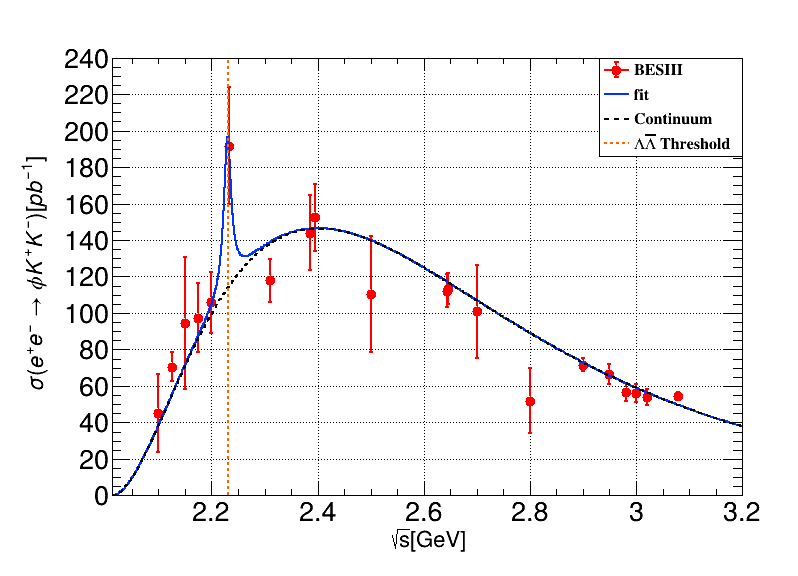
\includegraphics[width=0.8\textwidth]{figures/phikk.png}
      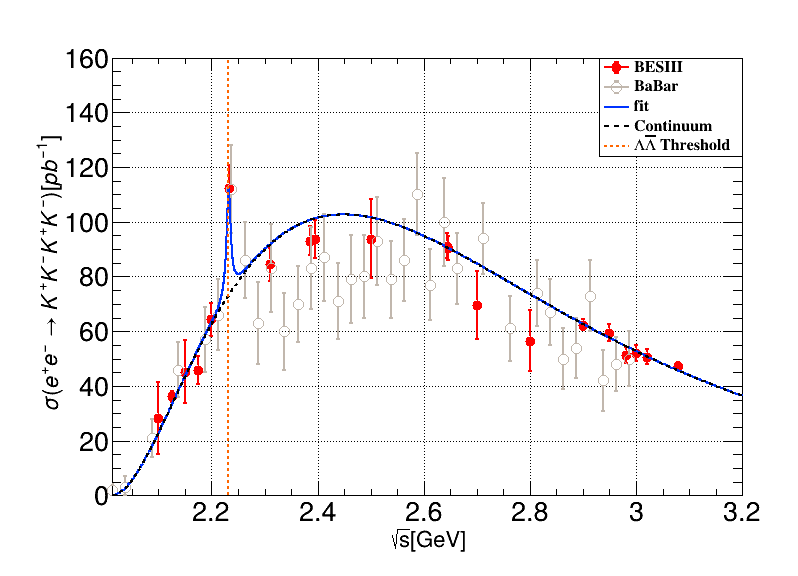
\includegraphics[width=0.8\textwidth]{figures/kkkk_nogreen.png}
    \end{column}
  \end{columns}
\end{frame}

\section{Data Sets}

\begin{frame}
  \frametitle{Data Sets}
	\begin{itemize}
    \item[$\star$] Data
    \begin{itemize}
    \item $\Upsilon(4S)$ : $360.531 fb^{-1}$
	  \item $\Upsilon(4S)$ off resonance :  $41.424 fb^{-1}$
	  \item $\Upsilon(5S)$ :  $19.34fb^{-1}$
    \item $\mathcal{L}_{tot} = 421.295\ \mathrm{fb}^{-1}$ (BaBar: $454\ \mathrm{fb}^{-1}$)
    \end{itemize}
    \item[$\star$] generic MC (MC15rd ,$\mathcal{L}_{gMC} = 4\mathcal{L}_{data}$)
    \begin{itemize}
      \item \texttt{/belle/collection/MC/MC15rd\_exp20-26\_4S\_v2}
      \item \texttt{/belle/collection/MC/MC15rd\_exp7-18\_4S\_v3}
    \end{itemize}
    \item[$\star$] SignalMC
    \begin{itemize}
      \item 10M run independent events generated by \texttt{PHOKHARA\_EvtGen}
    \end{itemize}
        \end{itemize}
\end{frame}

\section{Event Selection}

\begin{frame}
  \frametitle{Selection Criteria}
  \begin{columns}
    \begin{column}{0.5\textwidth}
      \begin{itemize}
        \item[$\star$] Charged track selection:
          \begin{itemize}
            \item $dr < 0.5$, $|dz| < 2$
            \item $N_{good} = 4$, $\sum Q = 0$
          \end{itemize}
        
        \item[$\star$] Photon selection:
          \begin{itemize}
            \item Select photon with highest energy
            \item $E \geq 3$ GeV
          \end{itemize}
          
        \item[$\star$] PID selection:
          \begin{itemize}
            \item $binaryPID = \frac{\mathcal{L}_{K}}{\mathcal{L}_k + \mathcal{L}_{\pi}} > 0.6$
            \item Number of good kaon $ \geq 3$
          \end{itemize}
          
        \item[$\star$] 3C kinematic fit:
          \begin{itemize}
            \item Event survives 3C fit
            \item $\chi^2 < 40$
          \end{itemize}
          
        \item[$\star$] $\phi$ mass window:
          \begin{itemize}
            \item $1.00133653 < M_{K^+K^-} < 1.03766347$
          \end{itemize}
          
        \item[$\star$] Select combination with minimum $\chi^2$
      \end{itemize}
    \end{column}
    \begin{column}{0.5\textwidth}
      \centering
      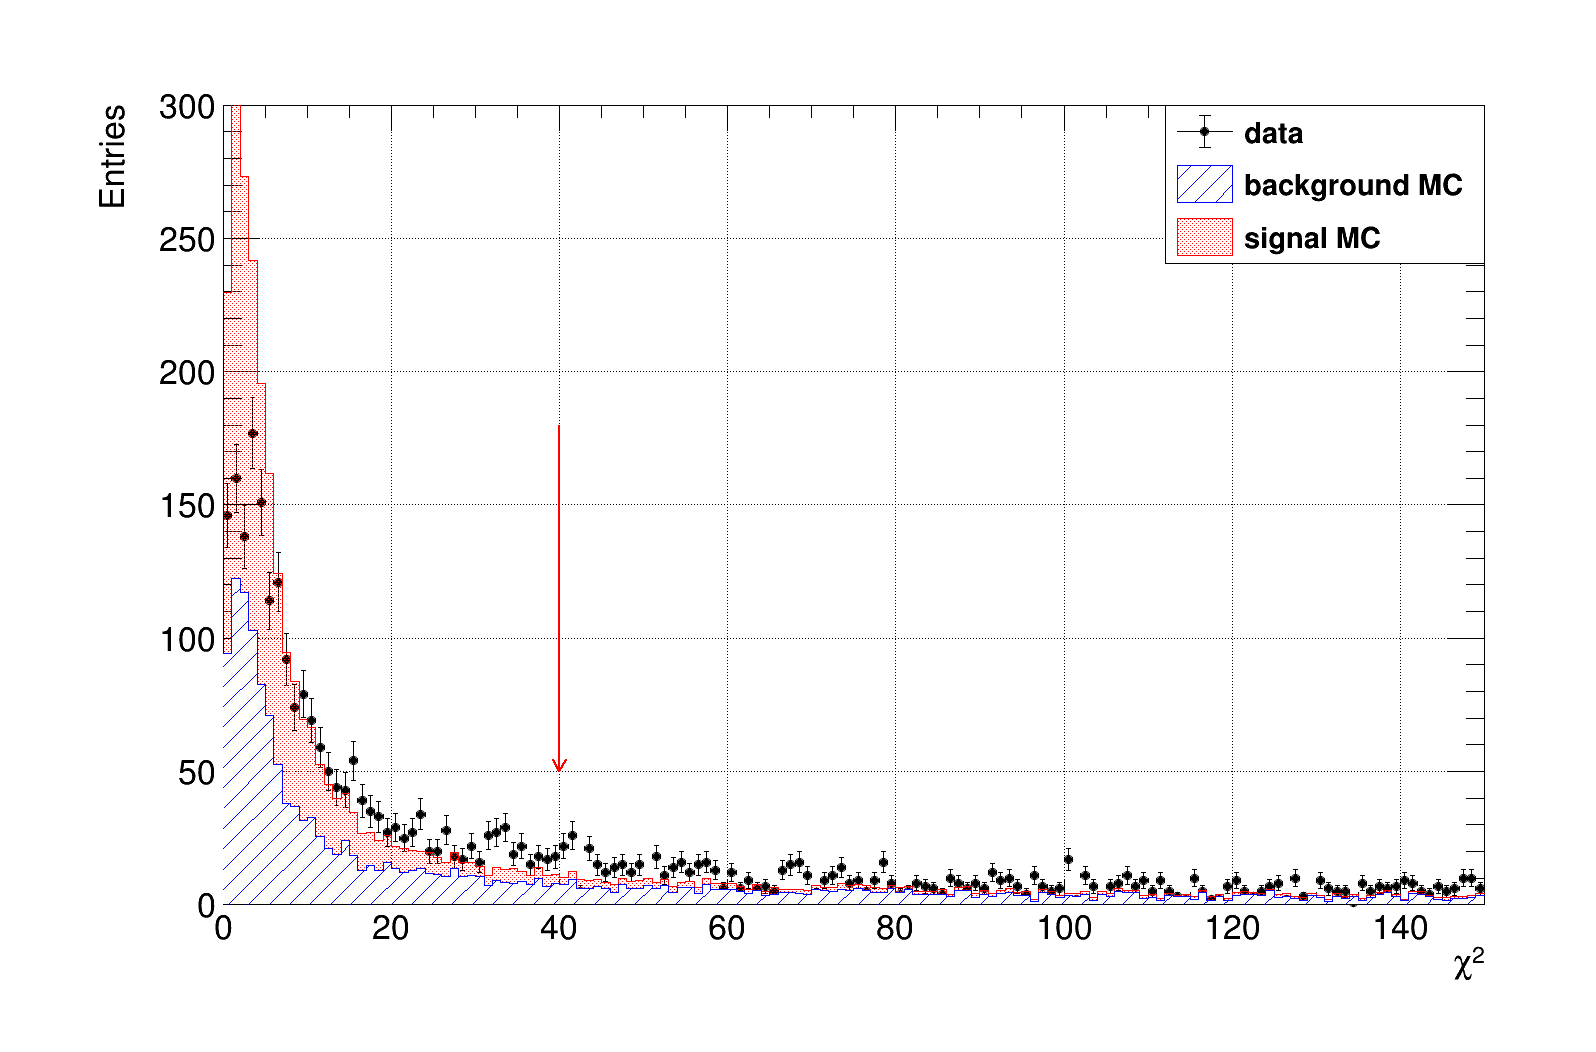
\includegraphics[width=0.75\textwidth]{figures/chisq_cut.png}
      
      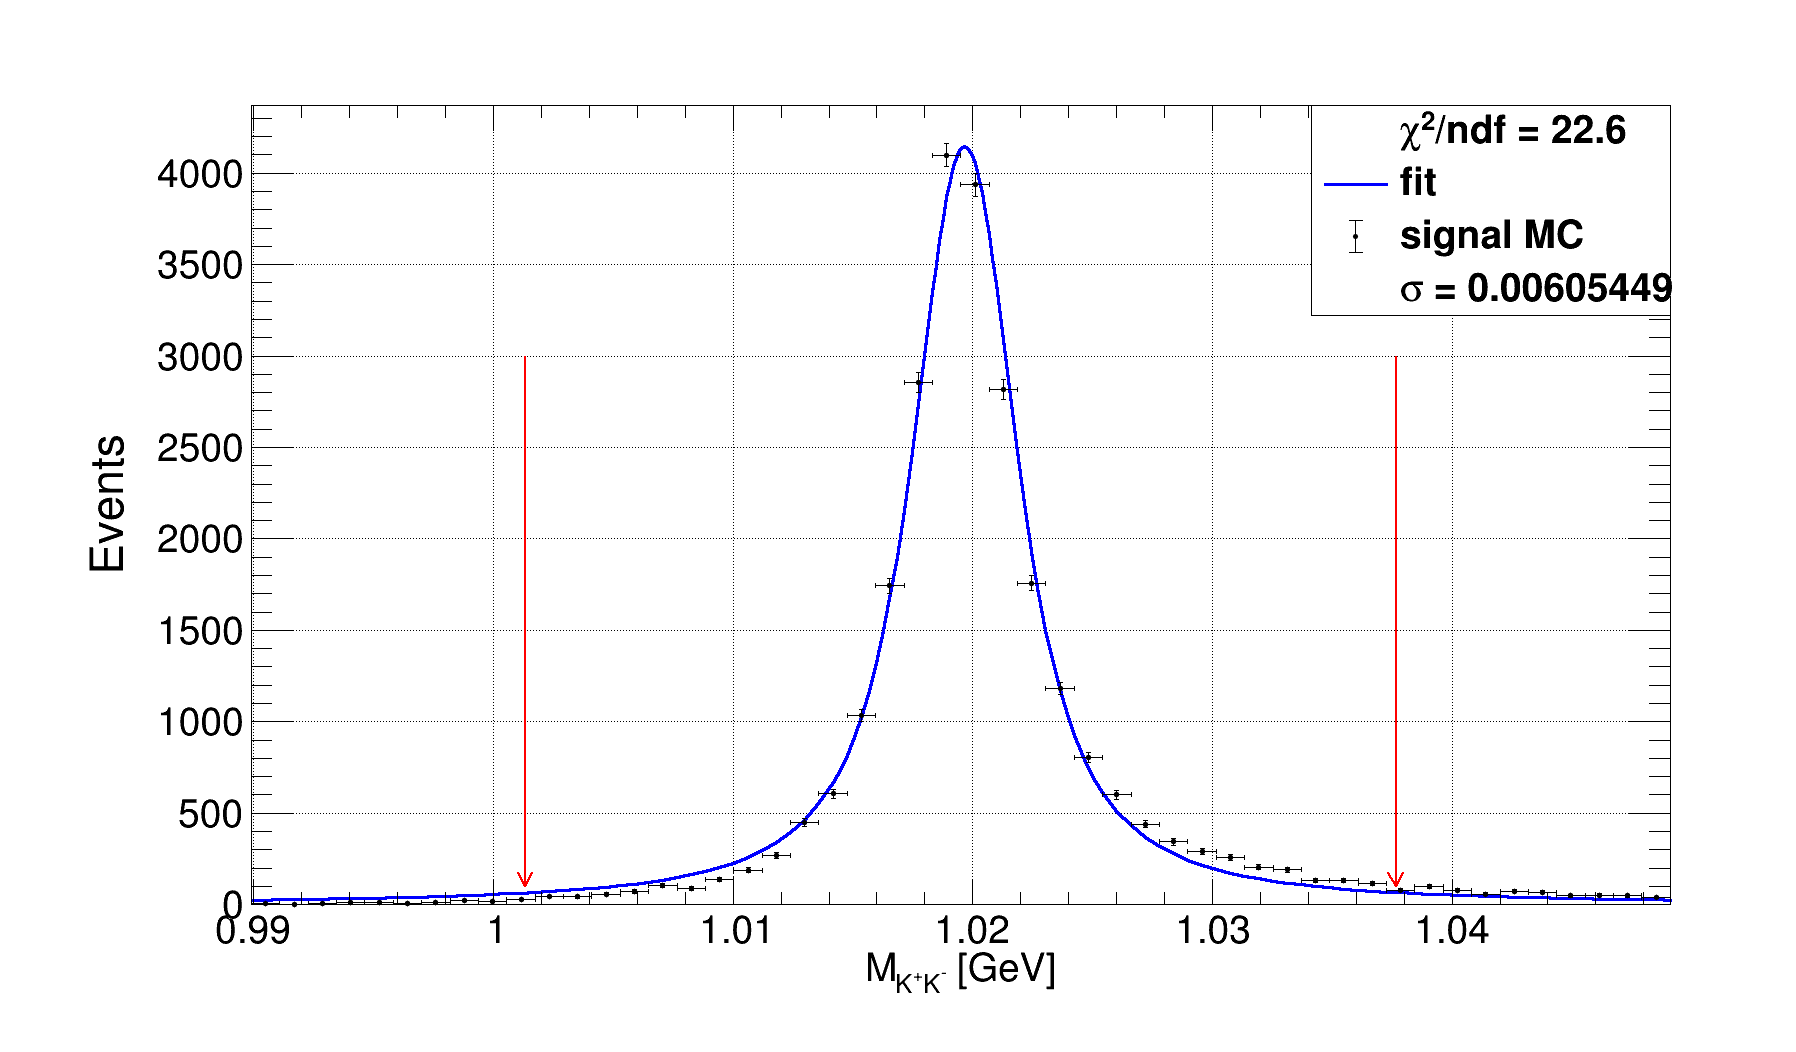
\includegraphics[width=0.75\textwidth]{figures/sMC_phi_fit_0.png}
    \end{column}
  \end{columns}
\end{frame}




\begin{frame}
  \frametitle{insert Line Shape}
  \begin{columns}[t]
    \begin{column}{1.5\textheight}
      \begin{columns}
        \begin{column}{0.3\textwidth}
          \centering
          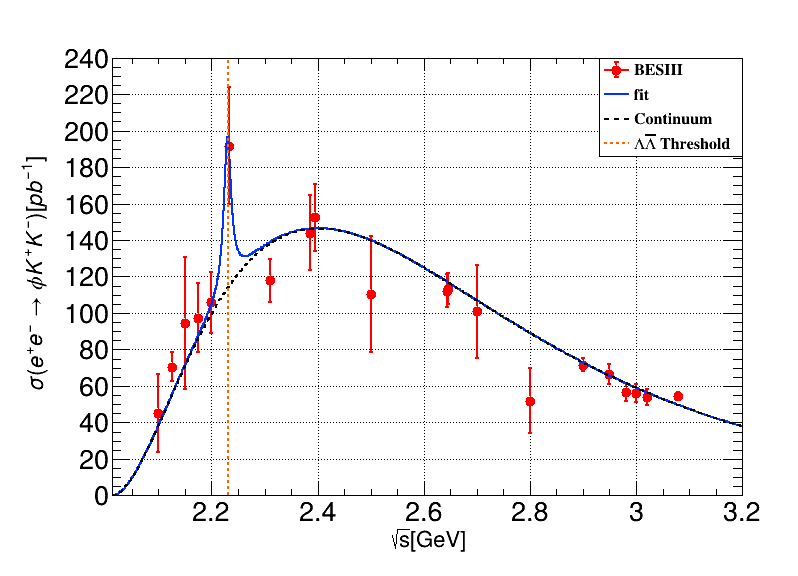
\includegraphics[width=\textwidth]{figures/phikk.png}
          \captionof{figure}{cross section}
        \end{column}
        \begin{column}{0.05\textwidth}
          \centering
          $\times$
        \end{column}
        \begin{column}{0.3\textwidth}
          \centering
          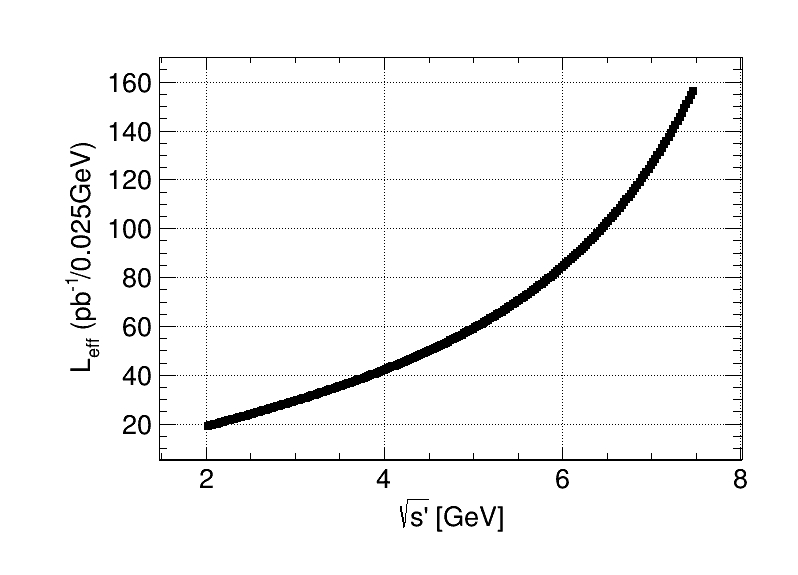
\includegraphics[width=\textwidth]{figures/eff_lumino.png}
          \captionof{figure}{effective luminosity}
        \end{column}
        \begin{column}{0.05\textwidth}
          \centering
          $=$
        \end{column}
        \begin{column}{0.3\textwidth}
          \centering
          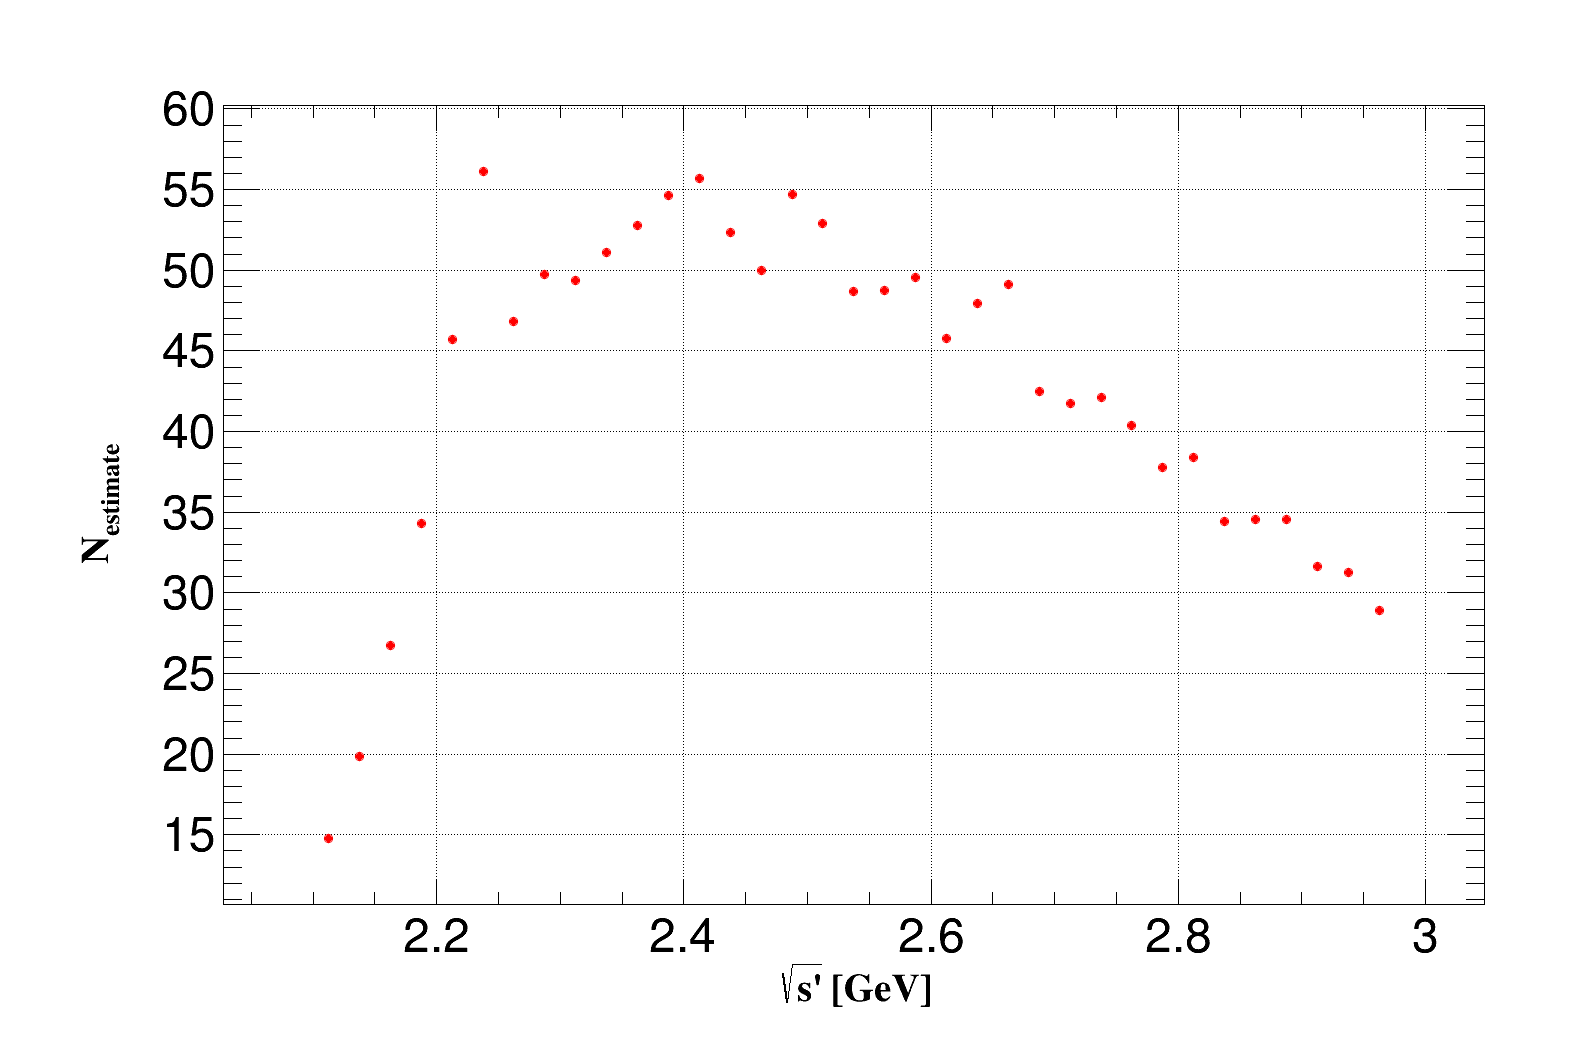
\includegraphics[width=\textwidth]{figures/Nes.png}
          \captionof{figure}{estimate entries}
        \end{column}
      \end{columns}
    \end{column}
  \end{columns}

  \vspace{0.5cm}

  \begin{columns}[t]
    \begin{column}{1.3\textheight}
      \begin{columns}
        \begin{column}{0.5\textwidth}
          \centering
          \begin{tikzpicture}[baseline=(current bounding box.center)]
            \node[anchor=west,inner sep=0] (image) at (0,0) {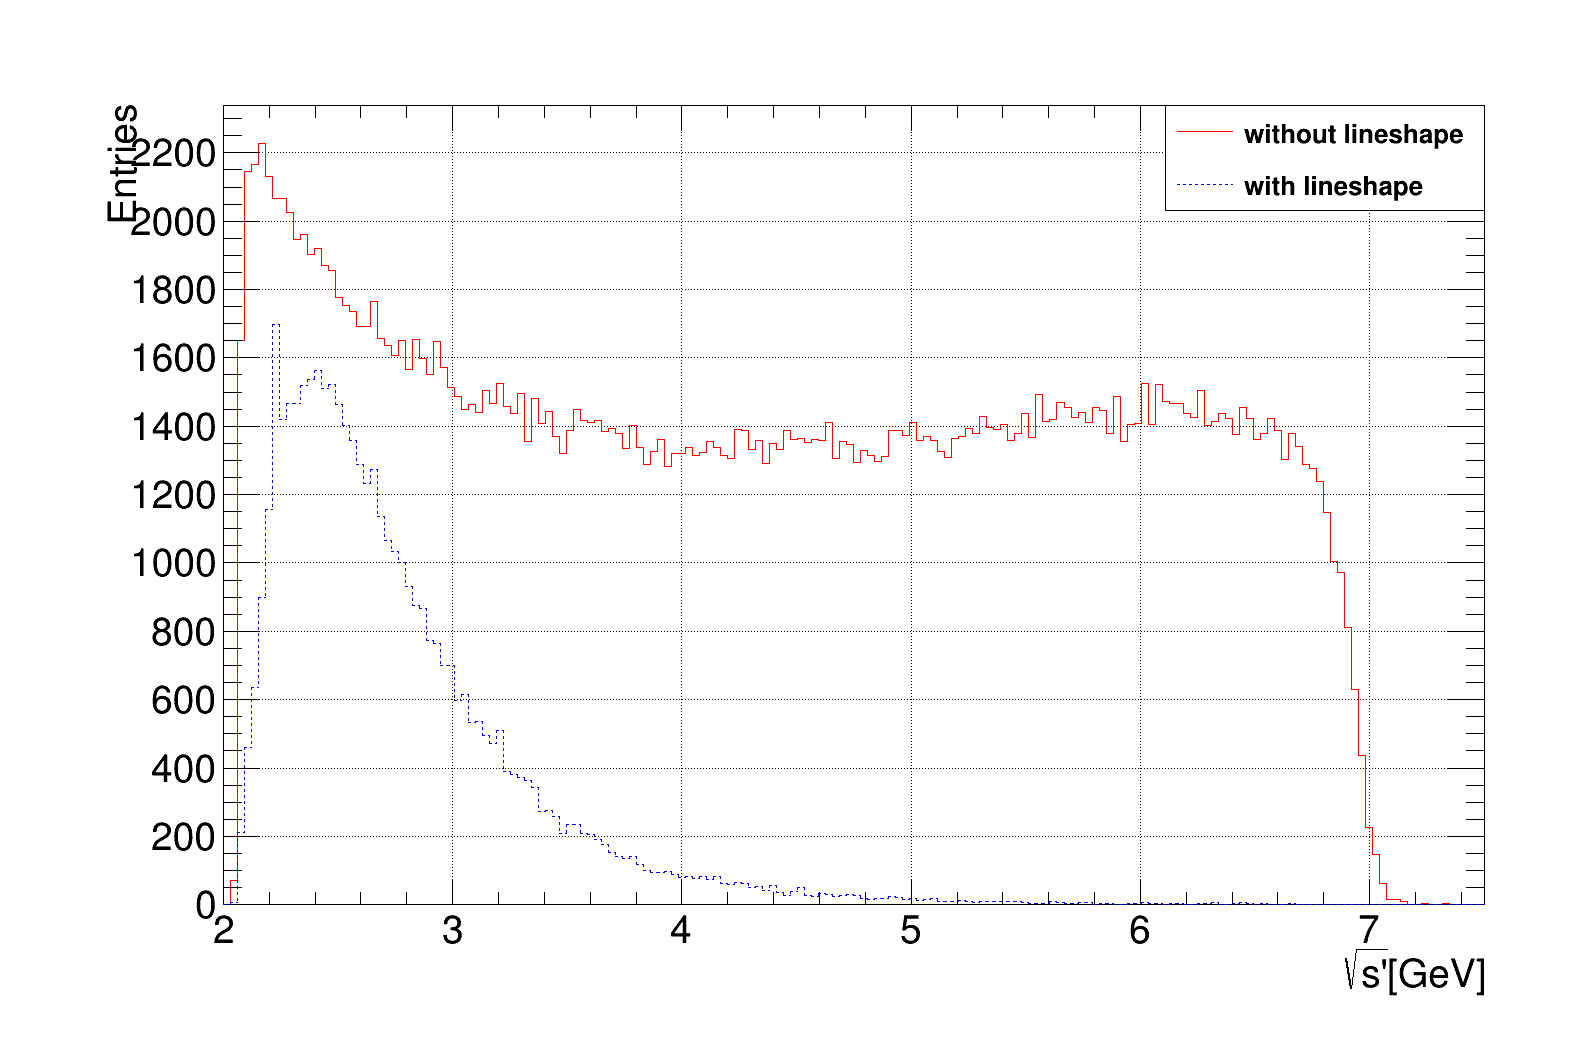
\includegraphics[width=0.8\textwidth]{figures/M_vpho.png}};
            \draw[->,thick,black] (-1.5,0.5) -- (-0.2,0.5);
          \end{tikzpicture}
        \end{column}
        \begin{column}{0.6\textwidth}
          \begin{itemize}
            \item $N_{estimate} =1495.38 $
            \item $N_{generate} =26350 , with \sqrt{s^{\prime}} < 3GeV$
            \item Normalization constant =  0.0567508
          \end{itemize}
        \end{column}
      \end{columns}
    \end{column}
  \end{columns}
\end{frame}

\begin{frame}
  \frametitle{Figure of Merit}
  \begin{columns}
    \begin{column}{0.33\textwidth}
      \centering
      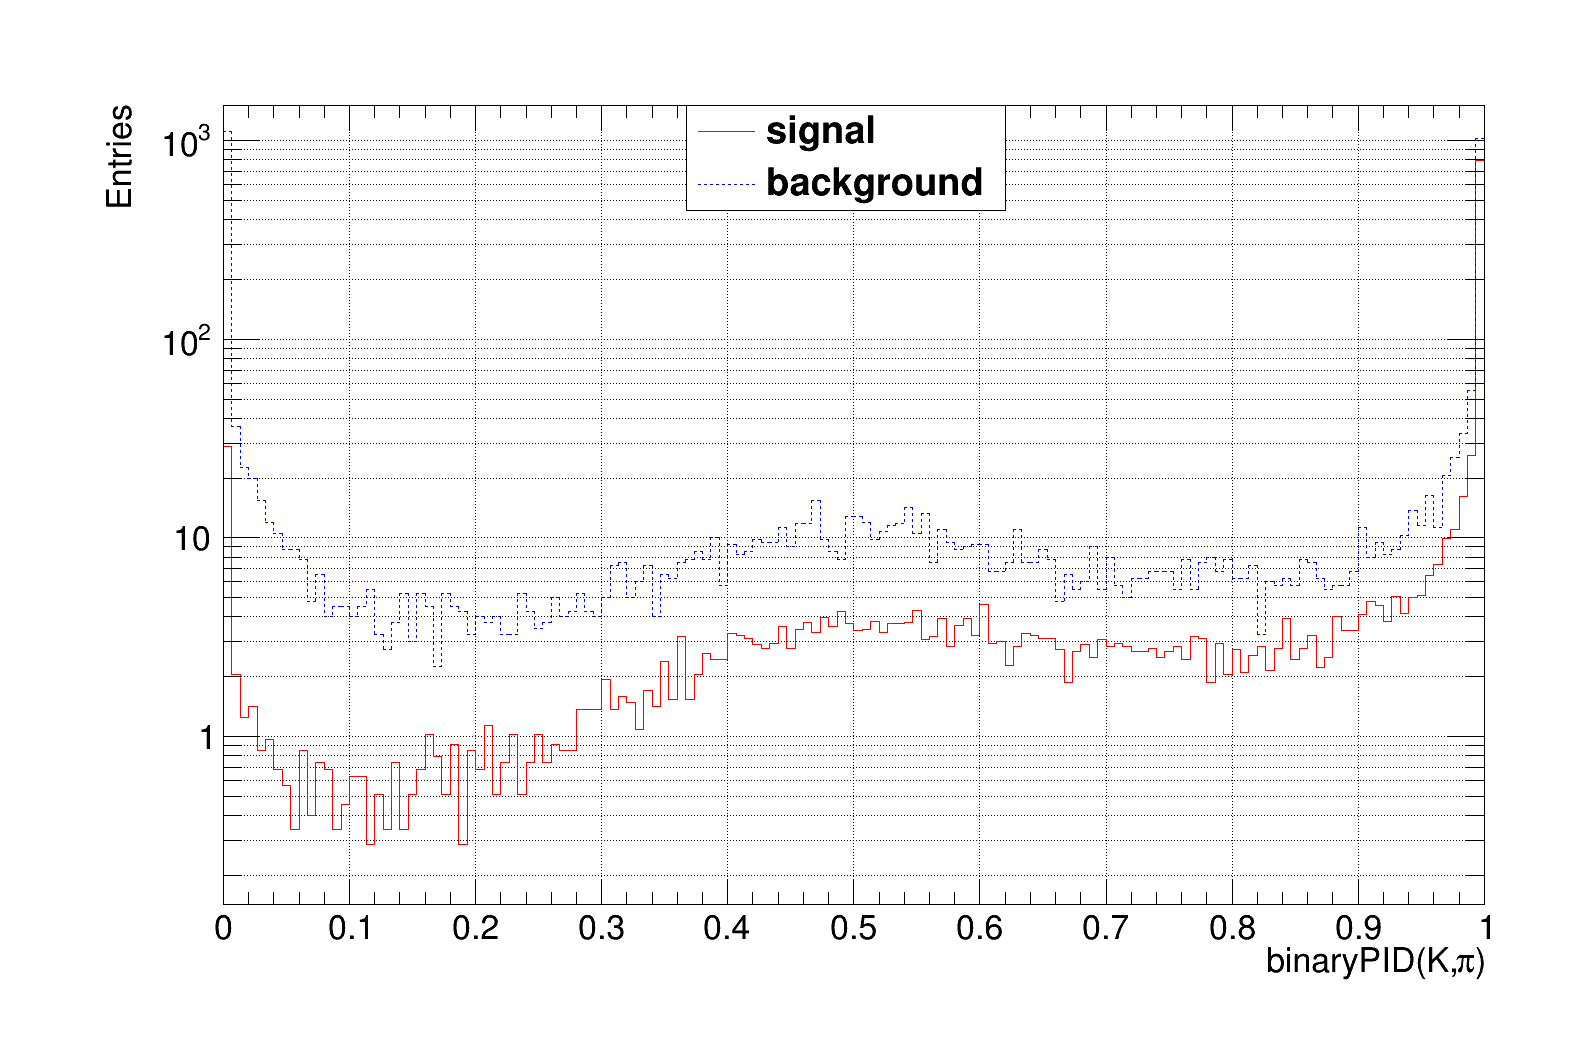
\includegraphics[width=\textwidth]{figures/binaryPID_phikp.png}
    \end{column}
    \begin{column}{0.33\textwidth}
      \centering
      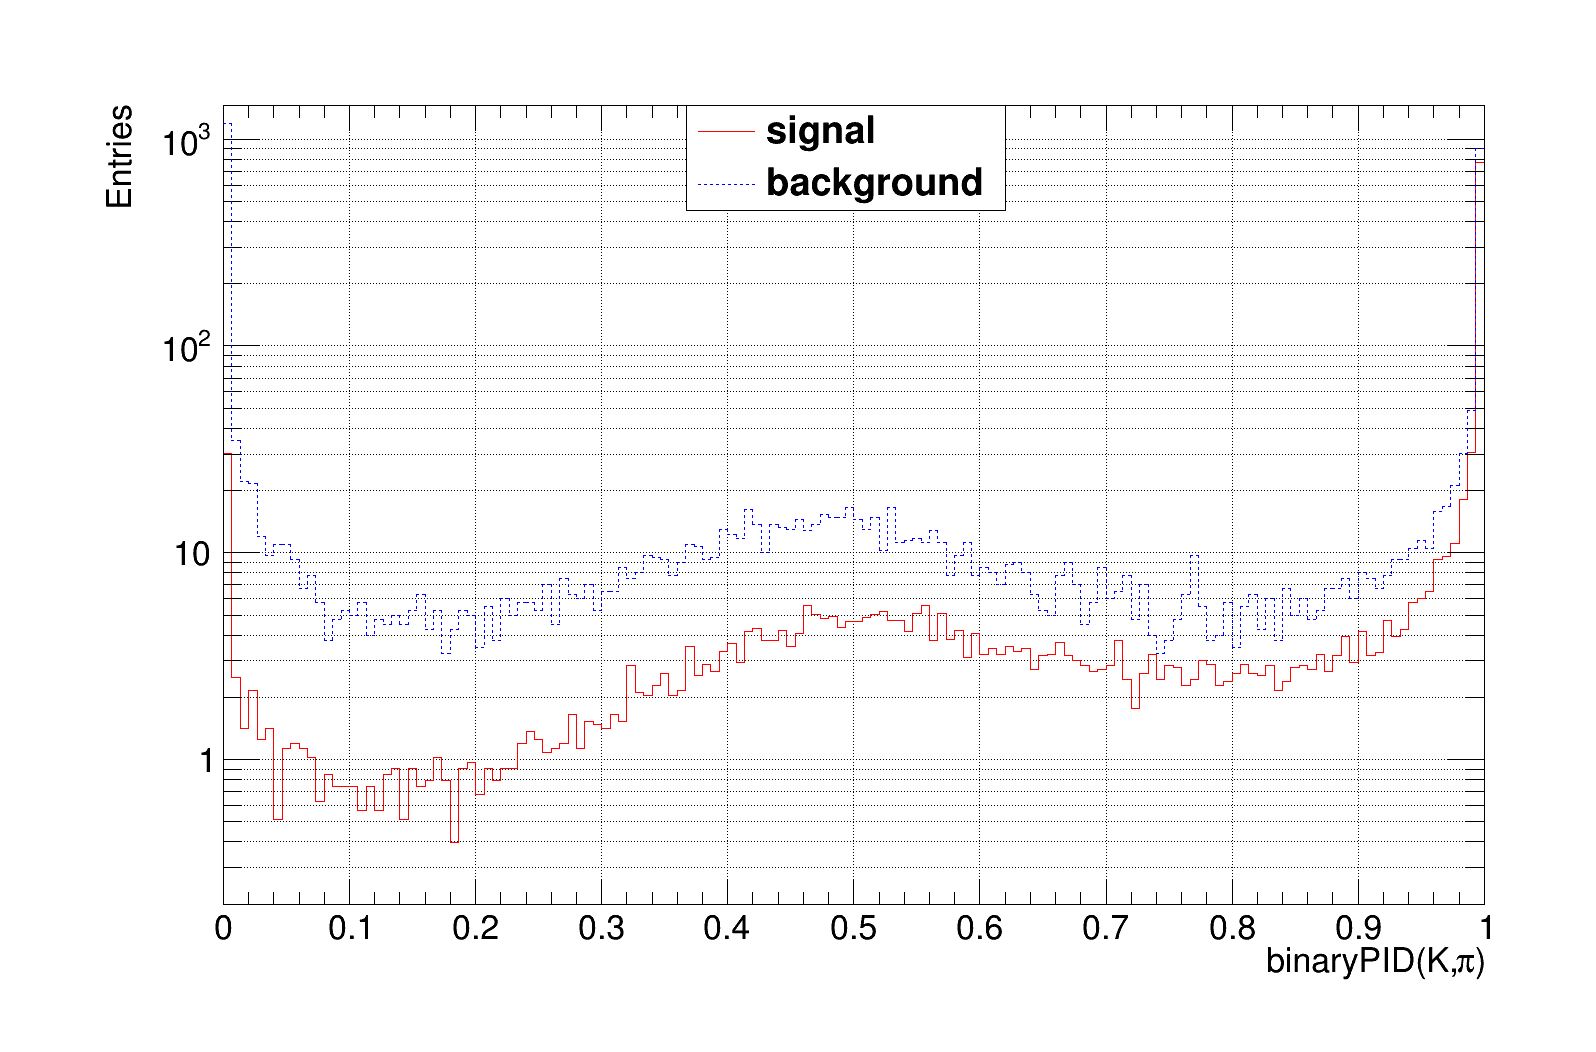
\includegraphics[width=\textwidth]{figures/binaryPID_eekp.png}
    \end{column}
    \begin{column}{0.33\textwidth}
      \centering
      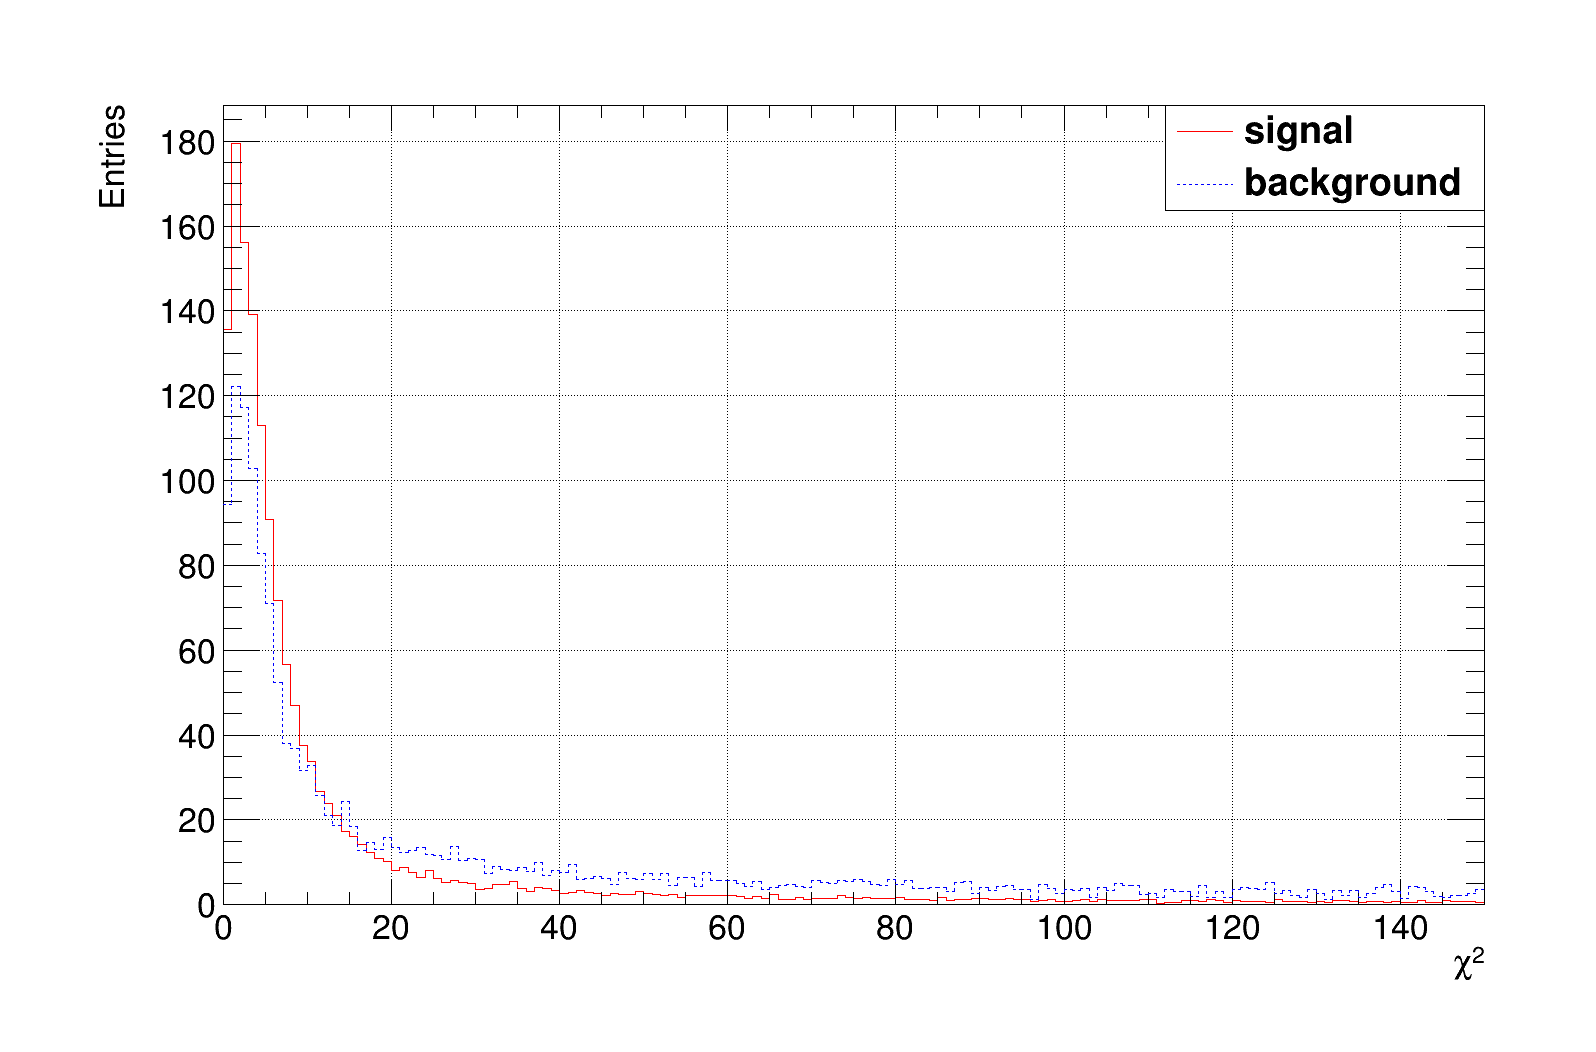
\includegraphics[width=\textwidth]{figures/chisq.png}
    \end{column}
  \end{columns}

  \begin{columns}
    \begin{column}{0.33\textwidth}
      \centering
      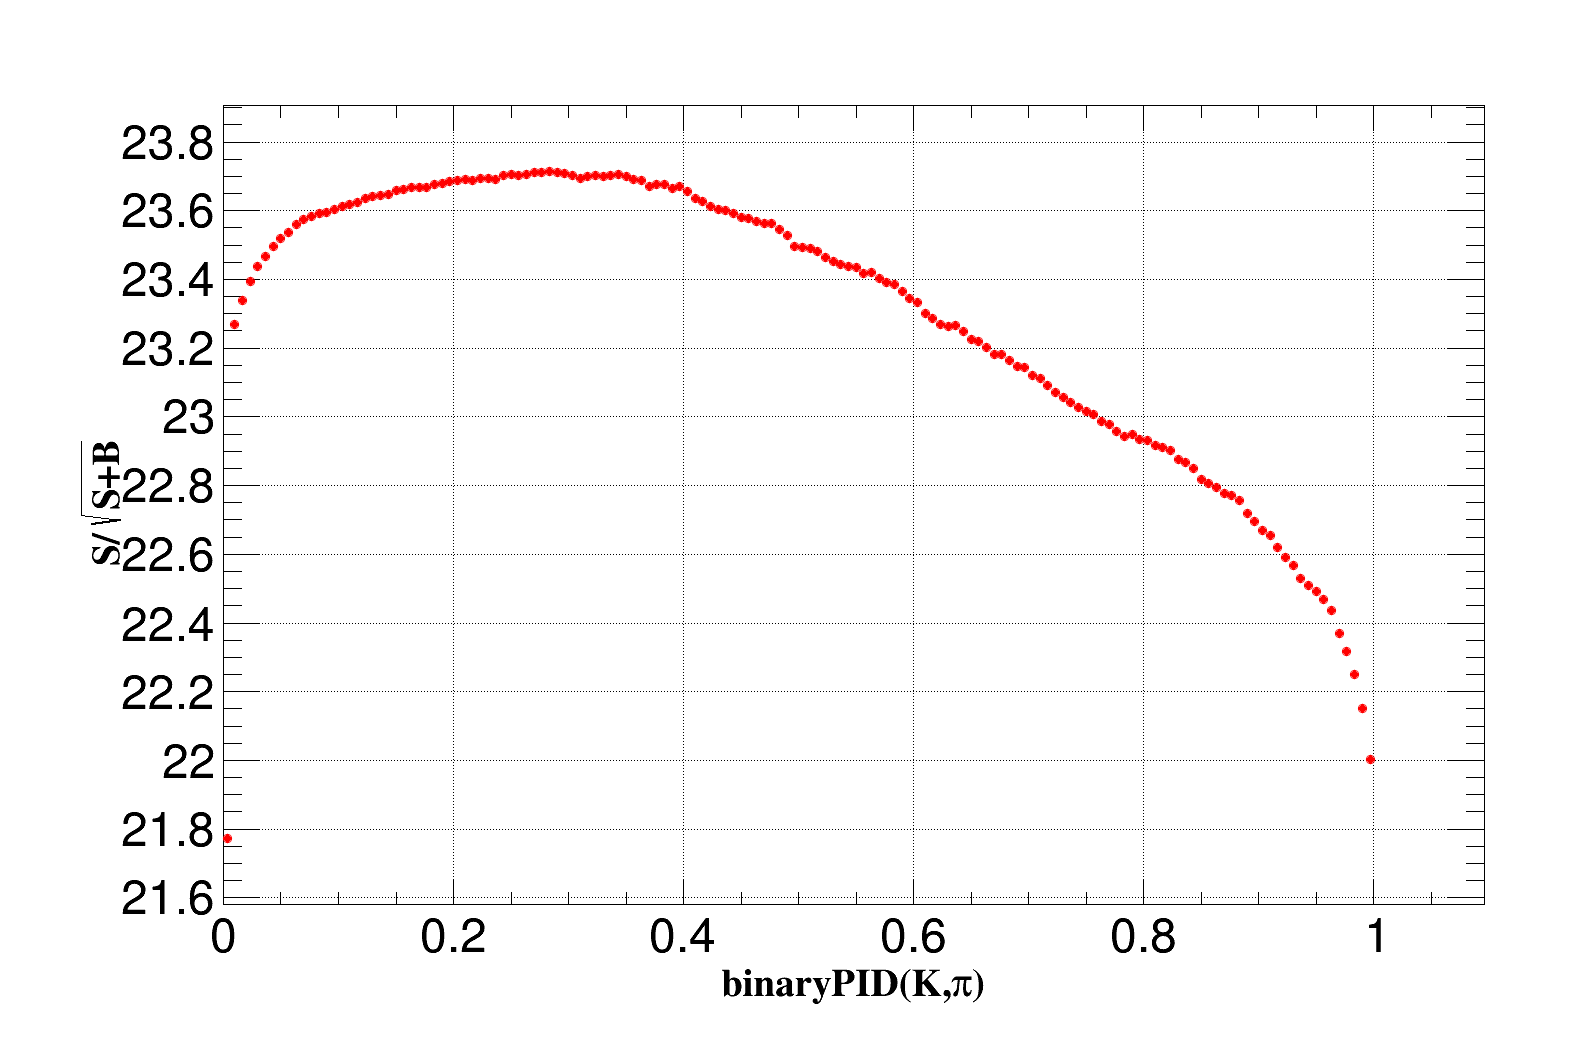
\includegraphics[width=\textwidth]{figures/binaryPID_phikp_fom.png}
      \captionof{figure}{binaryPID($K^+$ from $/phi$)}
    \end{column}
    \begin{column}{0.33\textwidth}
      \centering
      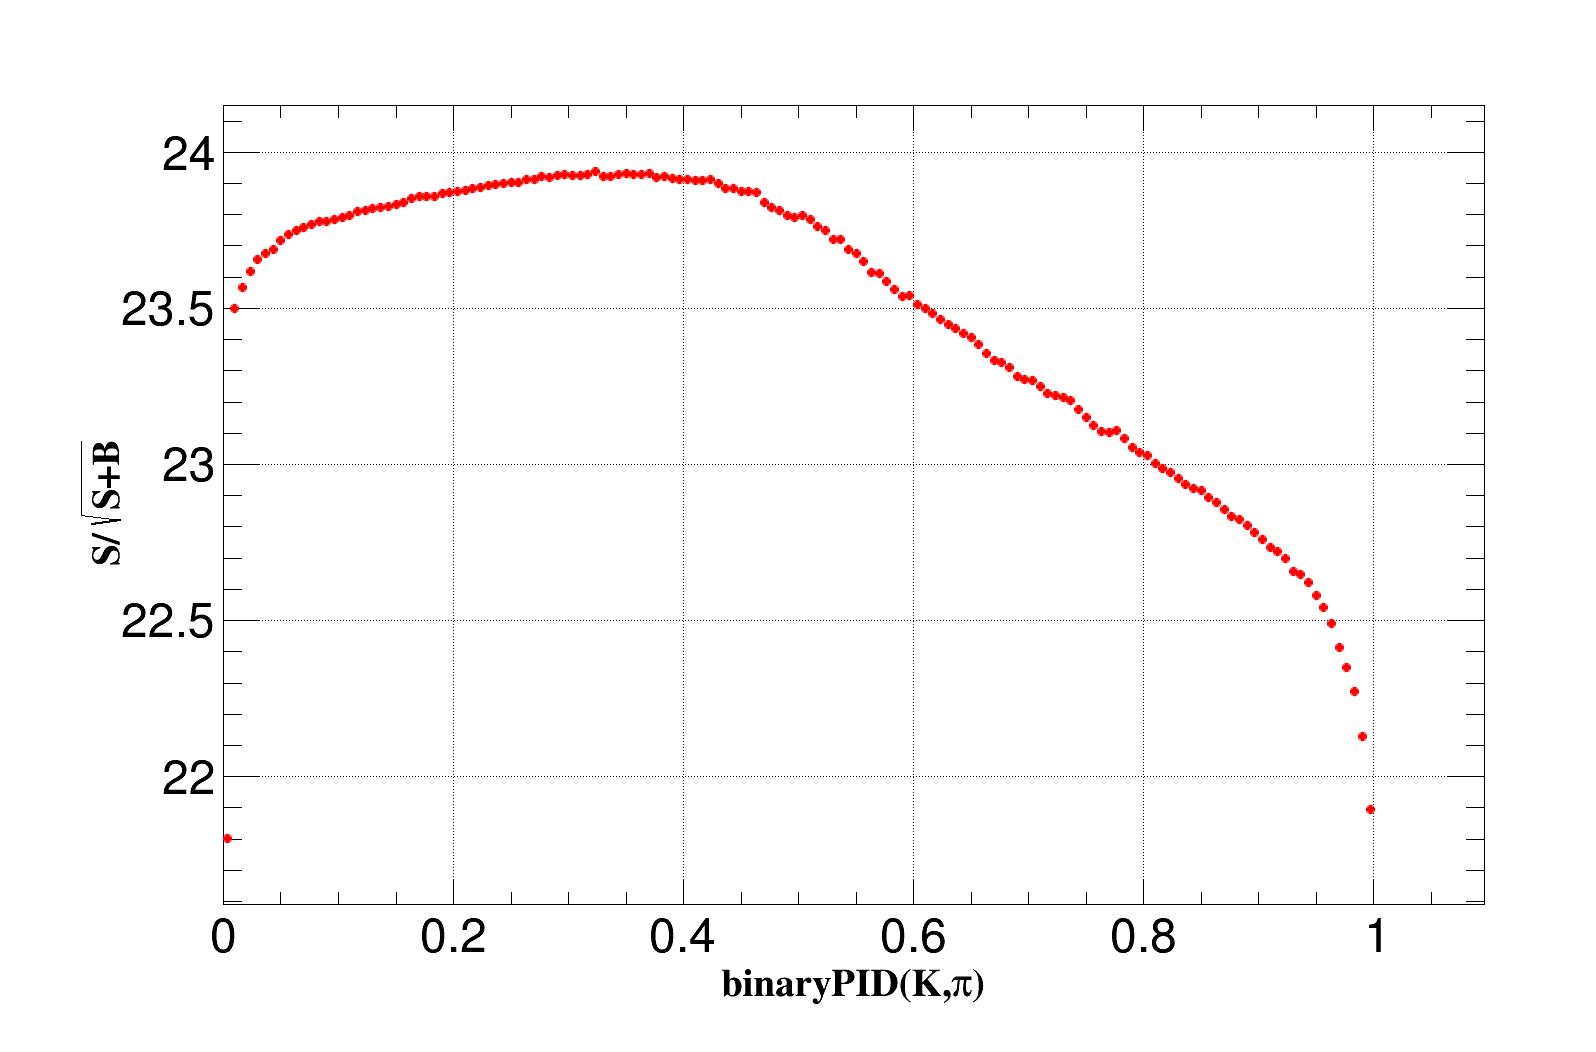
\includegraphics[width=\textwidth]{figures/binaryPID_eekp_fom.png}
      \captionof{figure}{binaryPID(the other $K^+$)}
    \end{column}
    \begin{column}{0.33\textwidth}
      \centering
      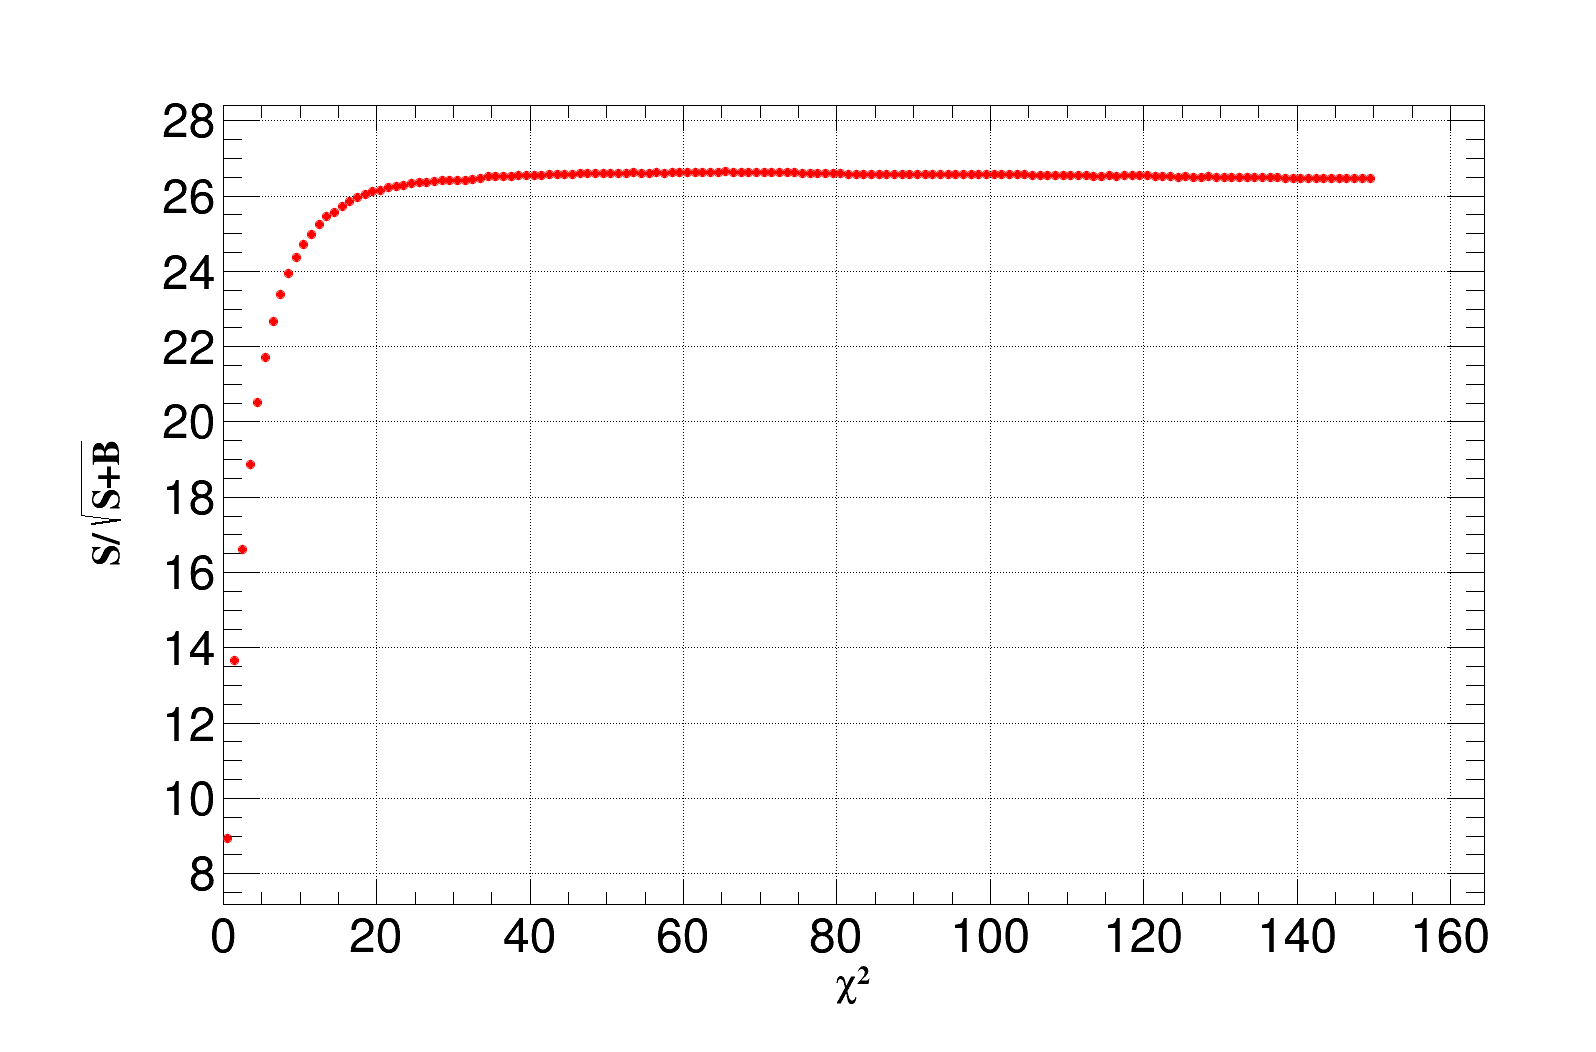
\includegraphics[width=\textwidth]{figures/chisq_fom.png}
      \captionof{figure}{$\chi^2$}
    \end{column}
  \end{columns}
\end{frame}


\section{Background study}
\begin{frame}
  \frametitle{Background study}
  \begin{columns}
    \begin{column}{0.5\textwidth}
      \centering
      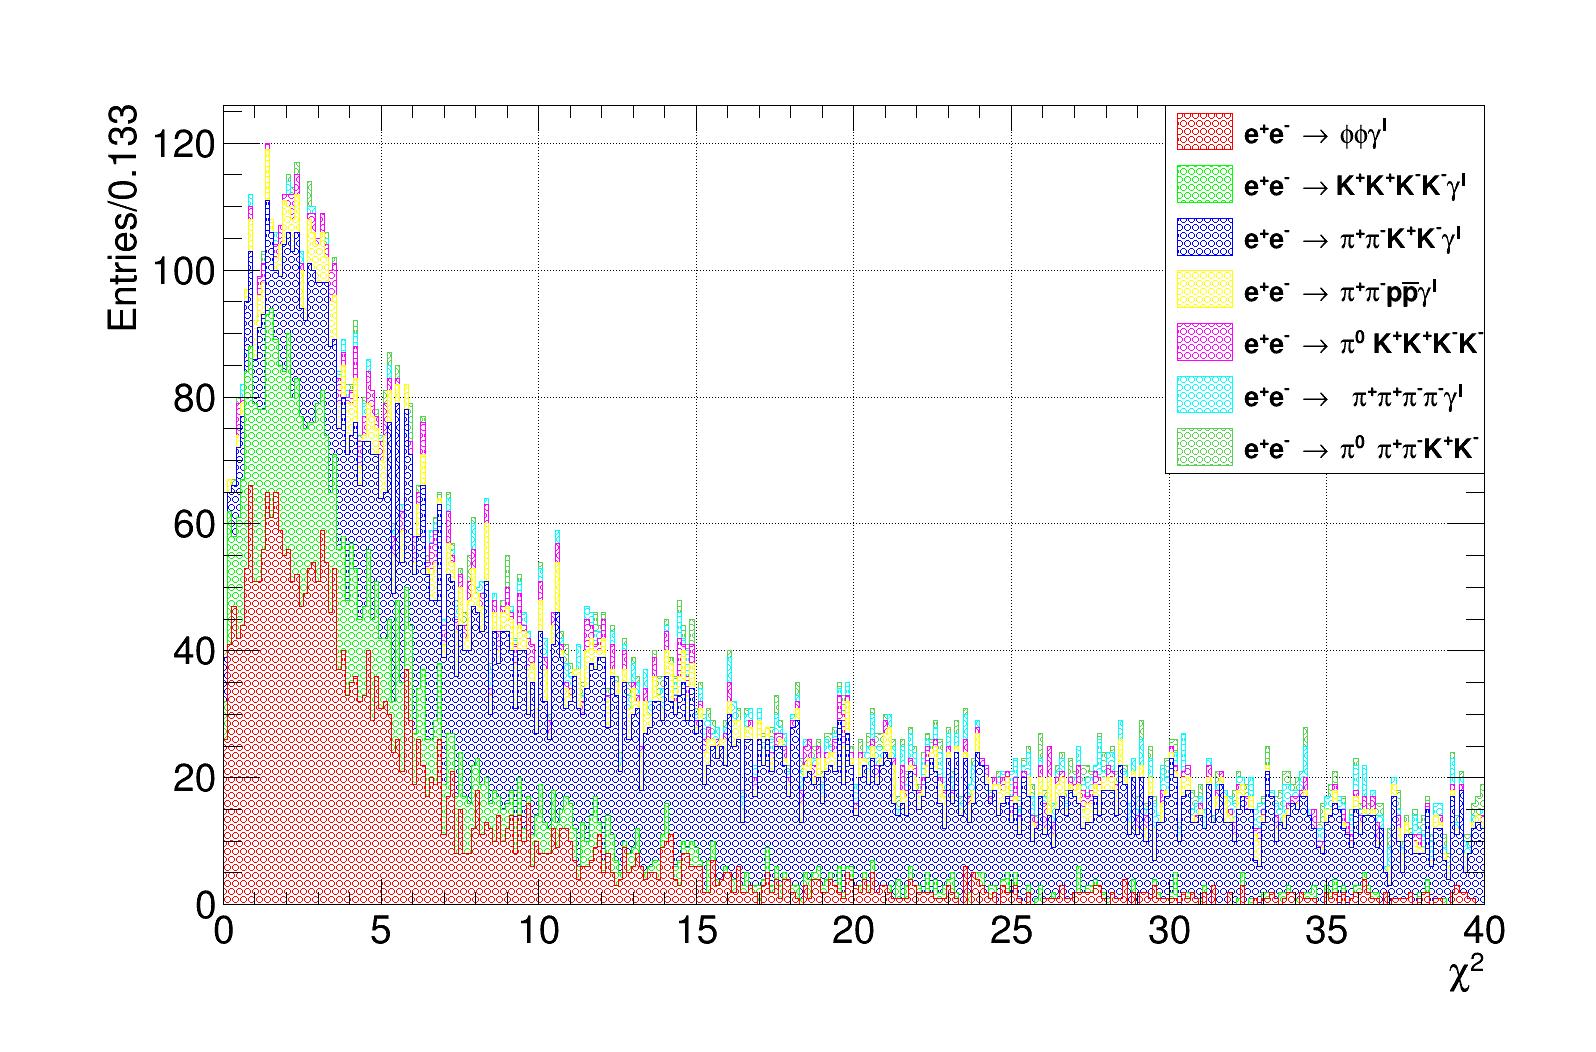
\includegraphics[width=0.8\textwidth]{figures/bkg_chisq.png}
    \end{column}
    \begin{column}{0.5\textwidth}
      \centering
      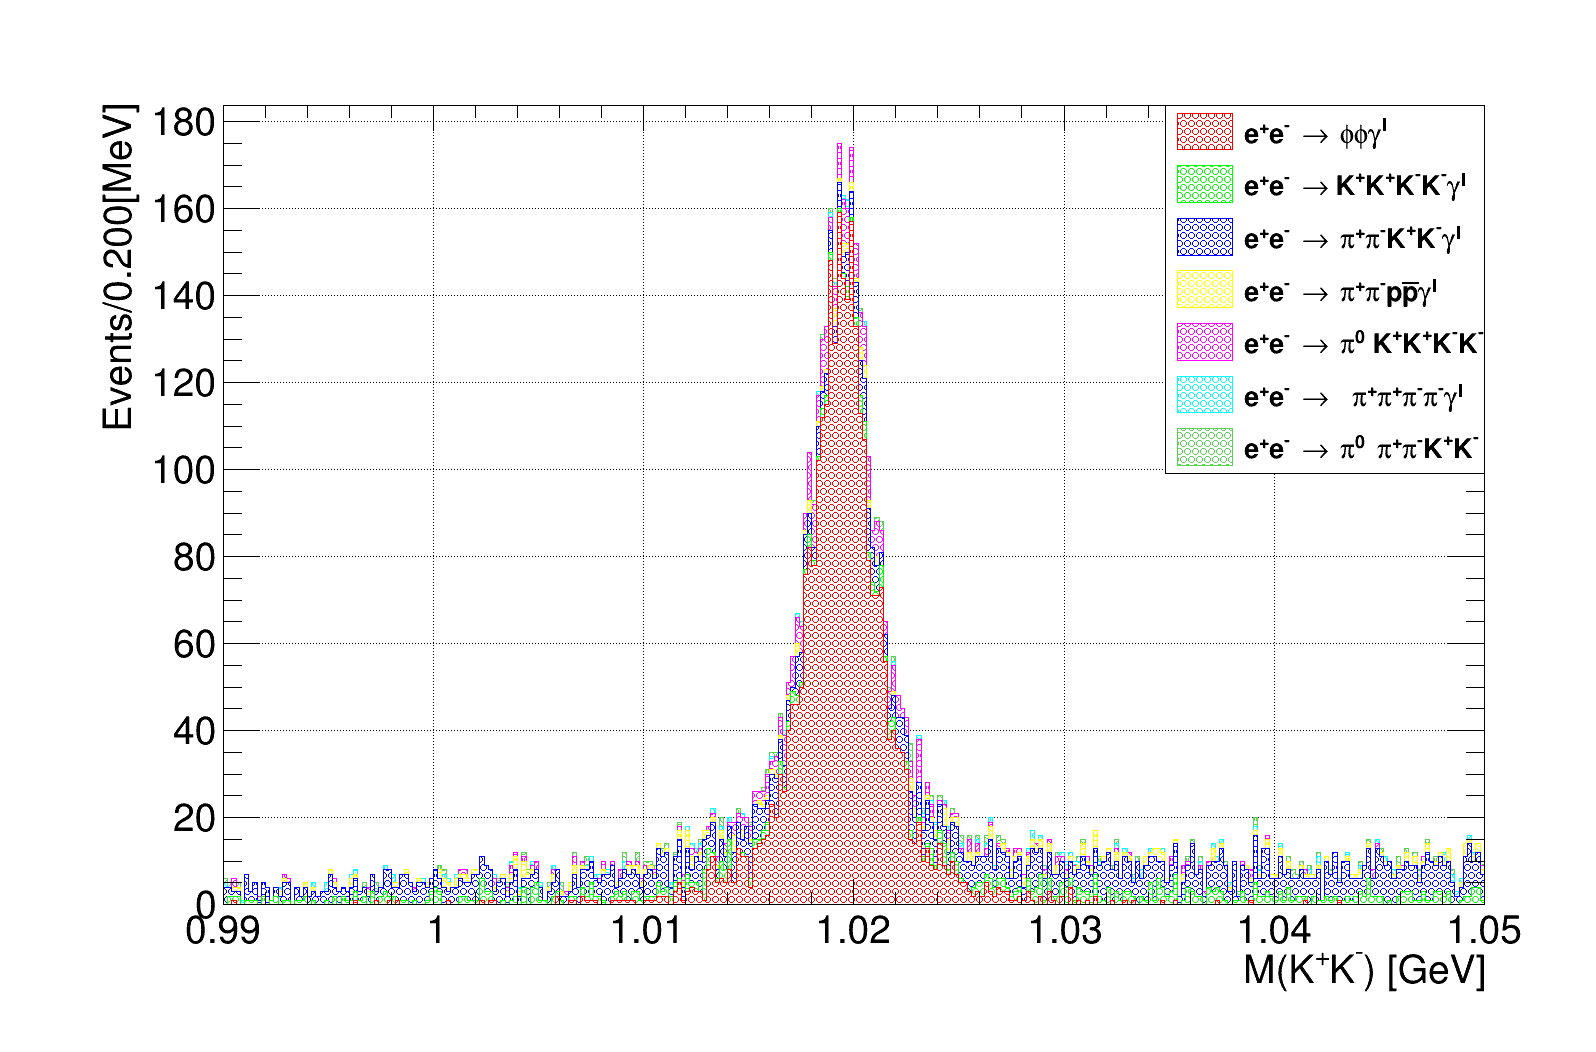
\includegraphics[width=0.8\textwidth]{figures/bkg_phi.png}
    \end{column}
  \end{columns}

  \begin{columns}
    \begin{column}{0.5\textwidth}
      \centering
      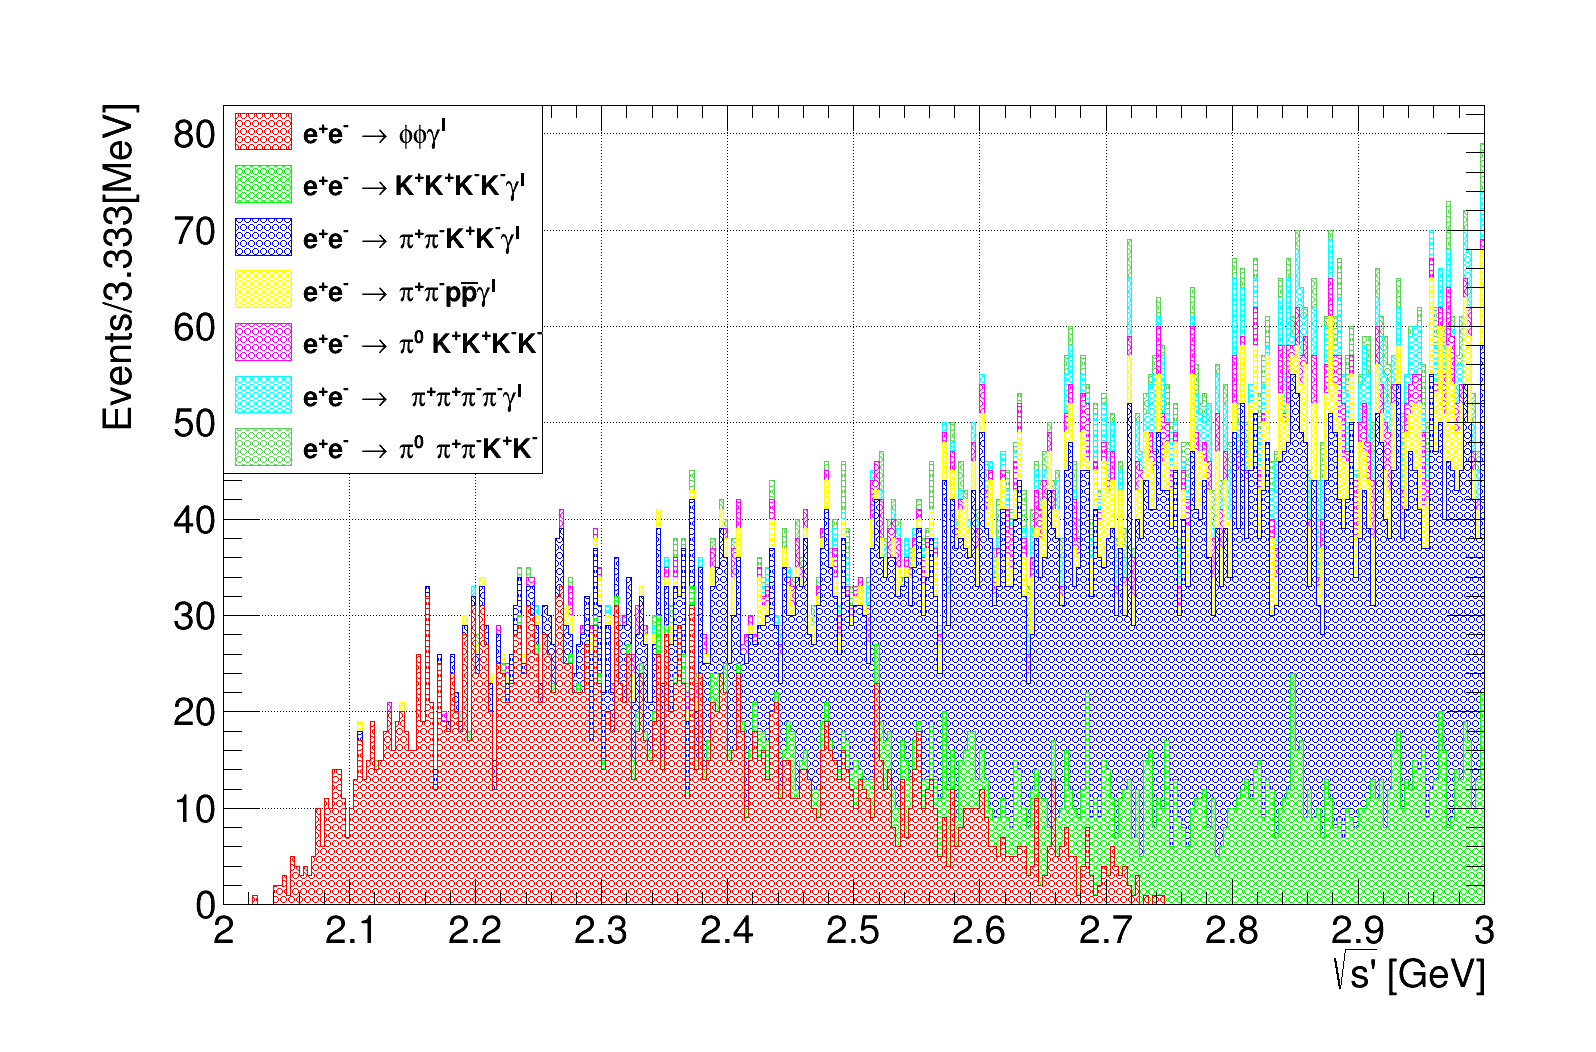
\includegraphics[width=0.8\textwidth]{figures/bkg_sqrts.png}
    \end{column}
    \begin{column}{0.5\textwidth}
      \centering
      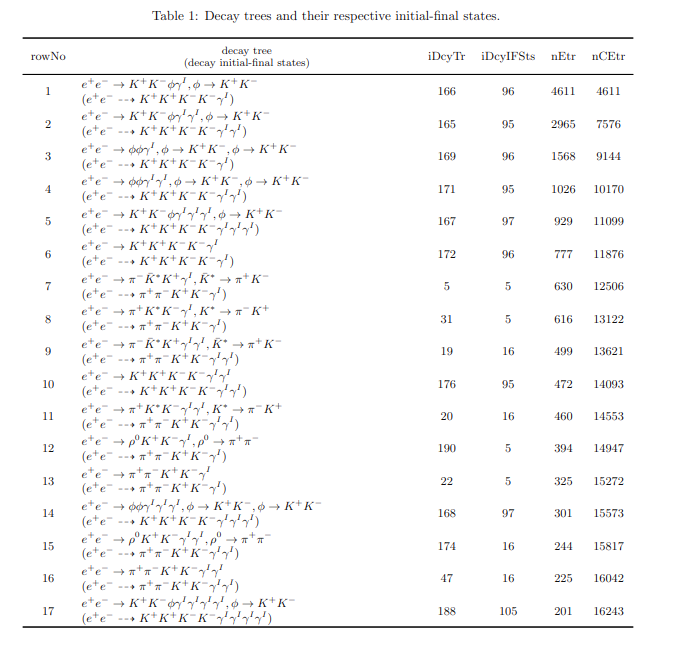
\includegraphics[width=0.6\textwidth]{figures/topo.png}
    \end{column}
  \end{columns}
\end{frame}

\section{cross section measurement}

\begin{frame}
  \frametitle{divide bin}
   \begin{columns}
    \begin{column}{0.4\textwidth}
      \centering
      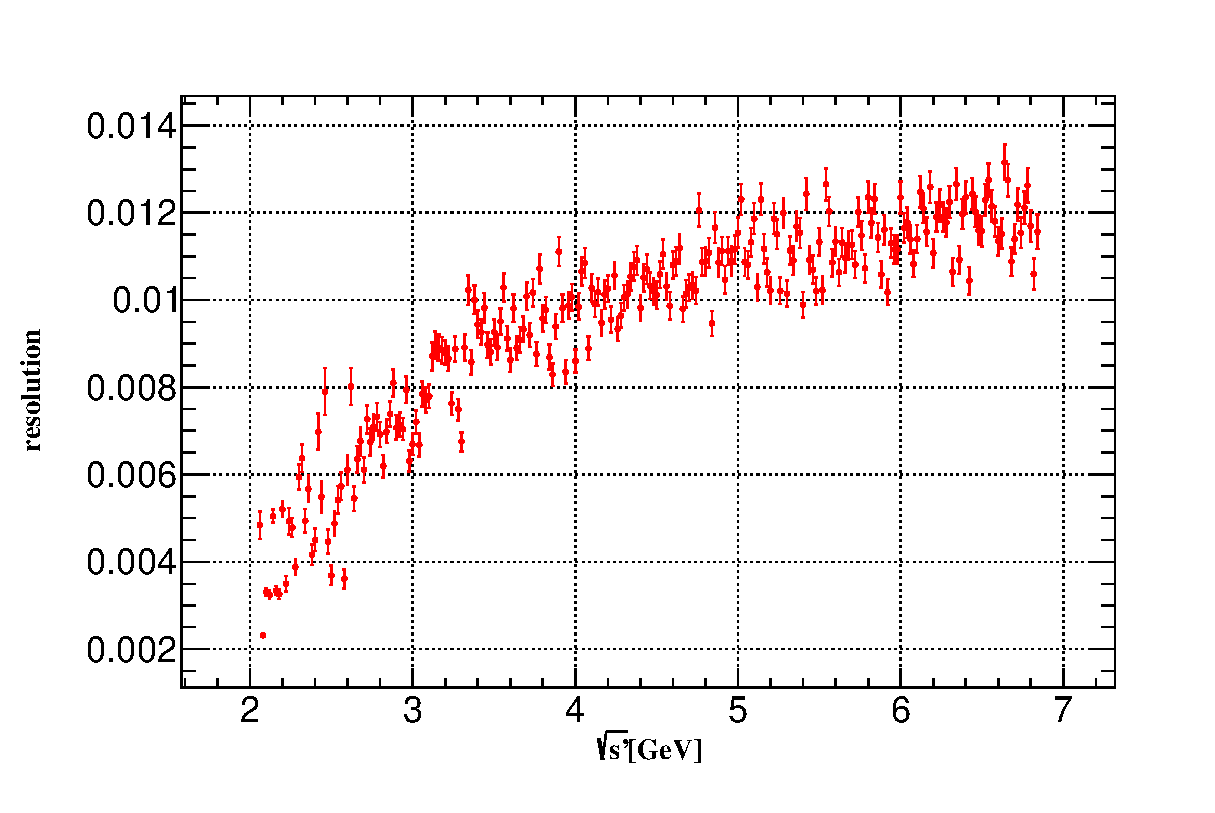
\includegraphics[width=\textwidth]{figures/divide_bin.eps}
    \end{column}

    \begin{column}{0.4\textwidth}
      \centering
      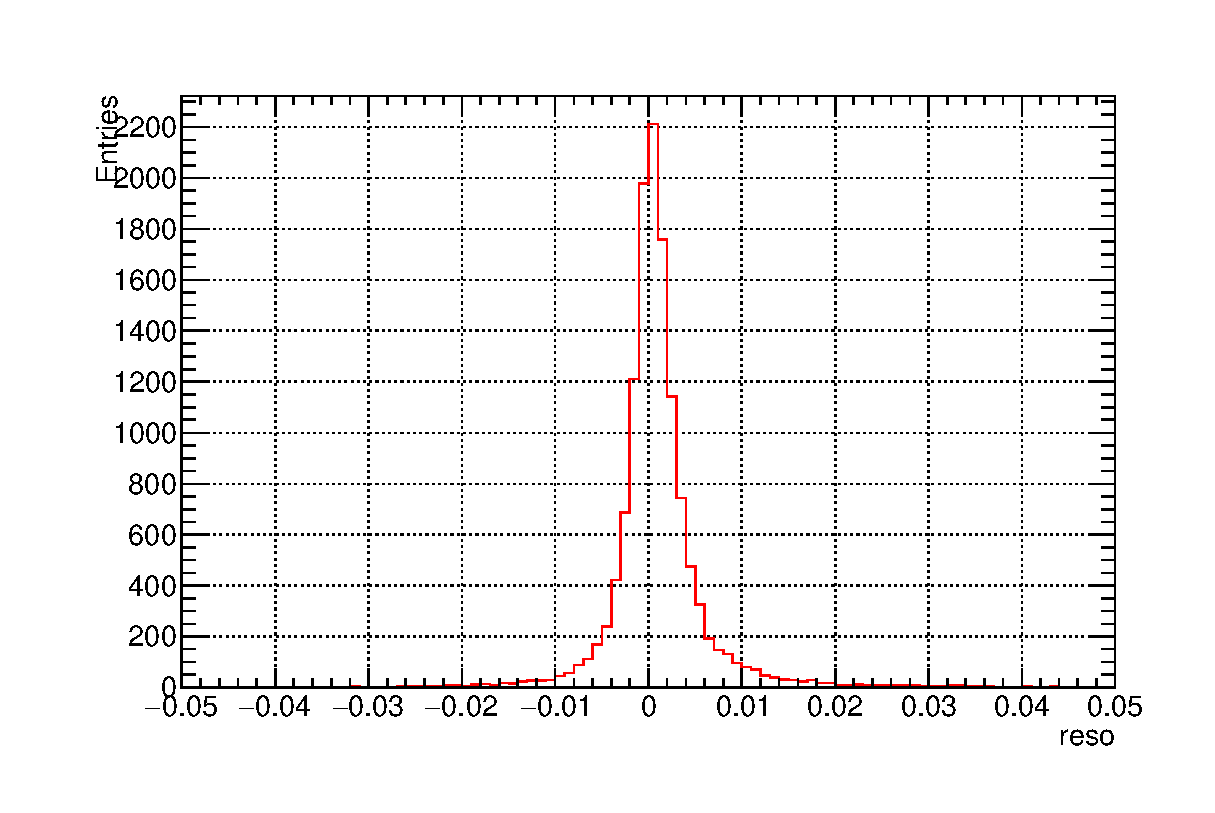
\includegraphics[width=\textwidth]{figures/reso.eps}
    \end{column}

    \begin{column}{0.33\textwidth}
      bin width:
     \begin{itemize}
      \item 25MeV at 2-3GeV
      \item 35MeV at 3-4.5GeV
      \item 40MeV at 4.5-7.5GeV
     \end{itemize}
    \end{column}
   \end{columns}
\end{frame}


\begin{frame}
  \frametitle{efficiency}
  using BW convolution a Guassian fit $\phi$ to get $N_{signal}$
 \begin{columns}
  \begin{column}{0.5\textwidth}
   \centering
   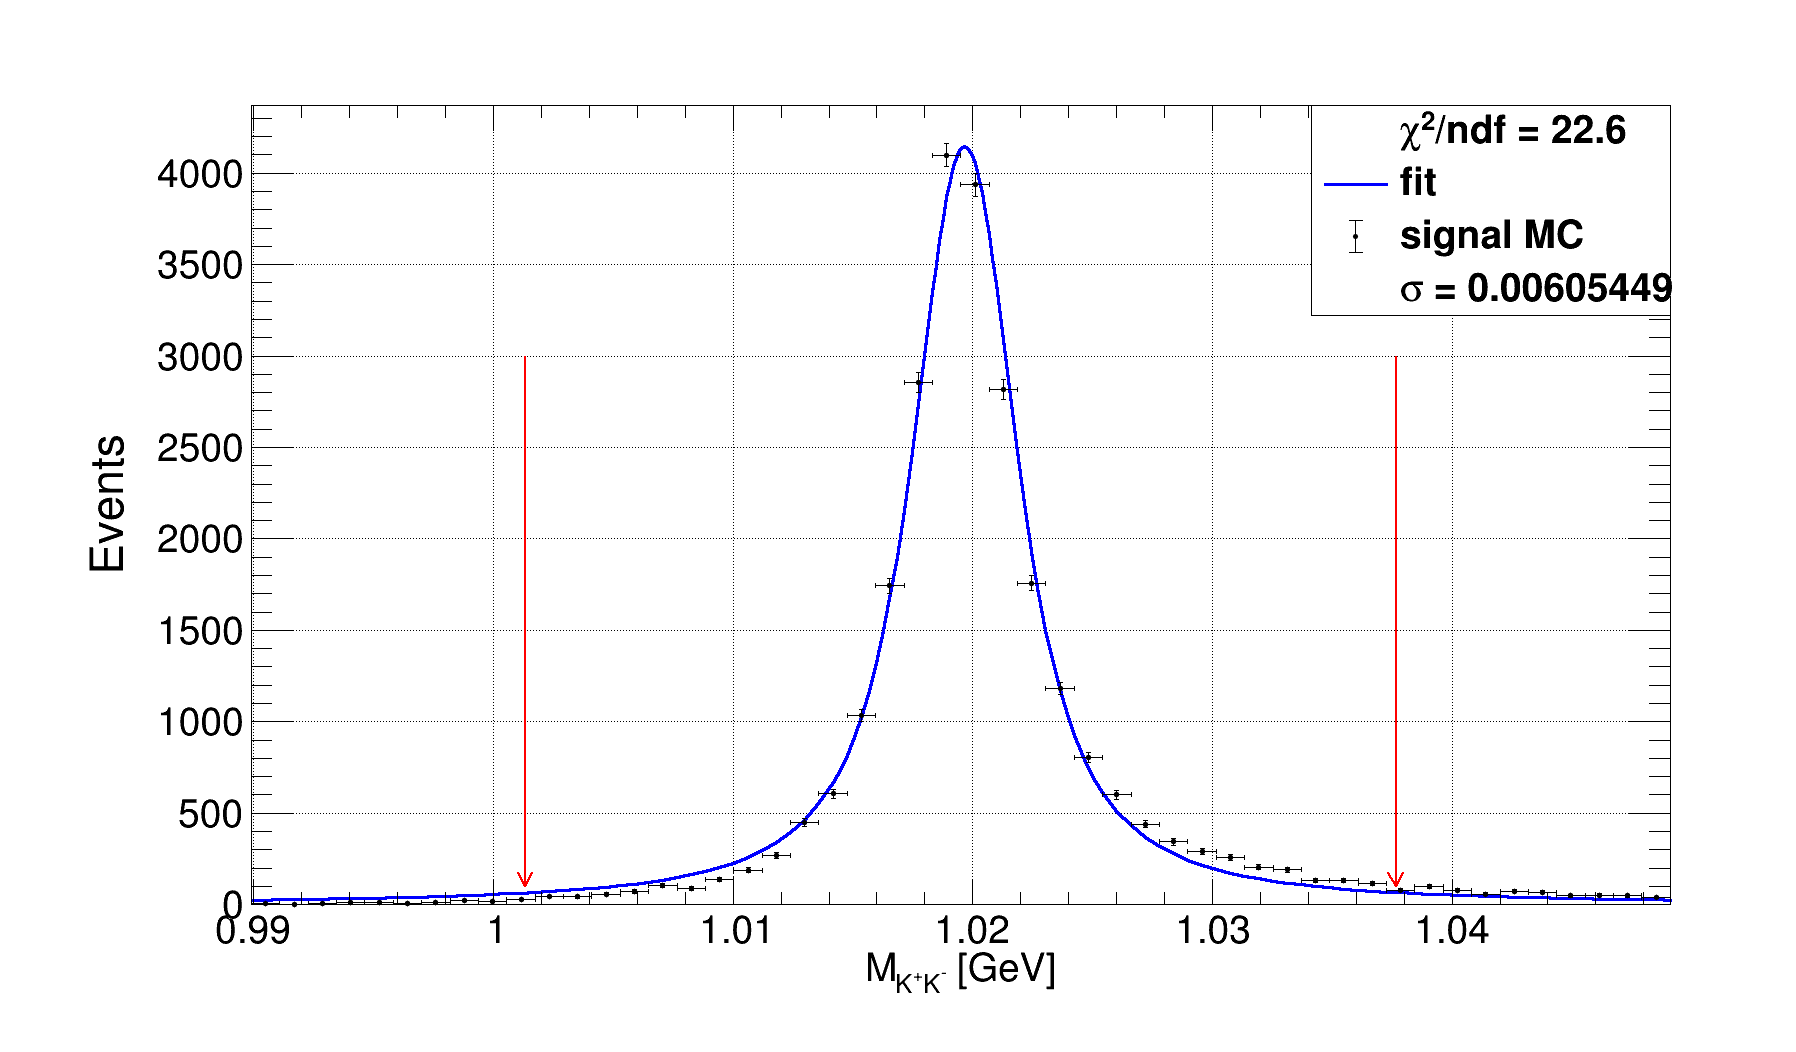
\includegraphics[width=\textwidth]{figures/sMC_phi_fit_0.png}
  \end{column}

  \begin{column}{0.5\textwidth}
   \centering
   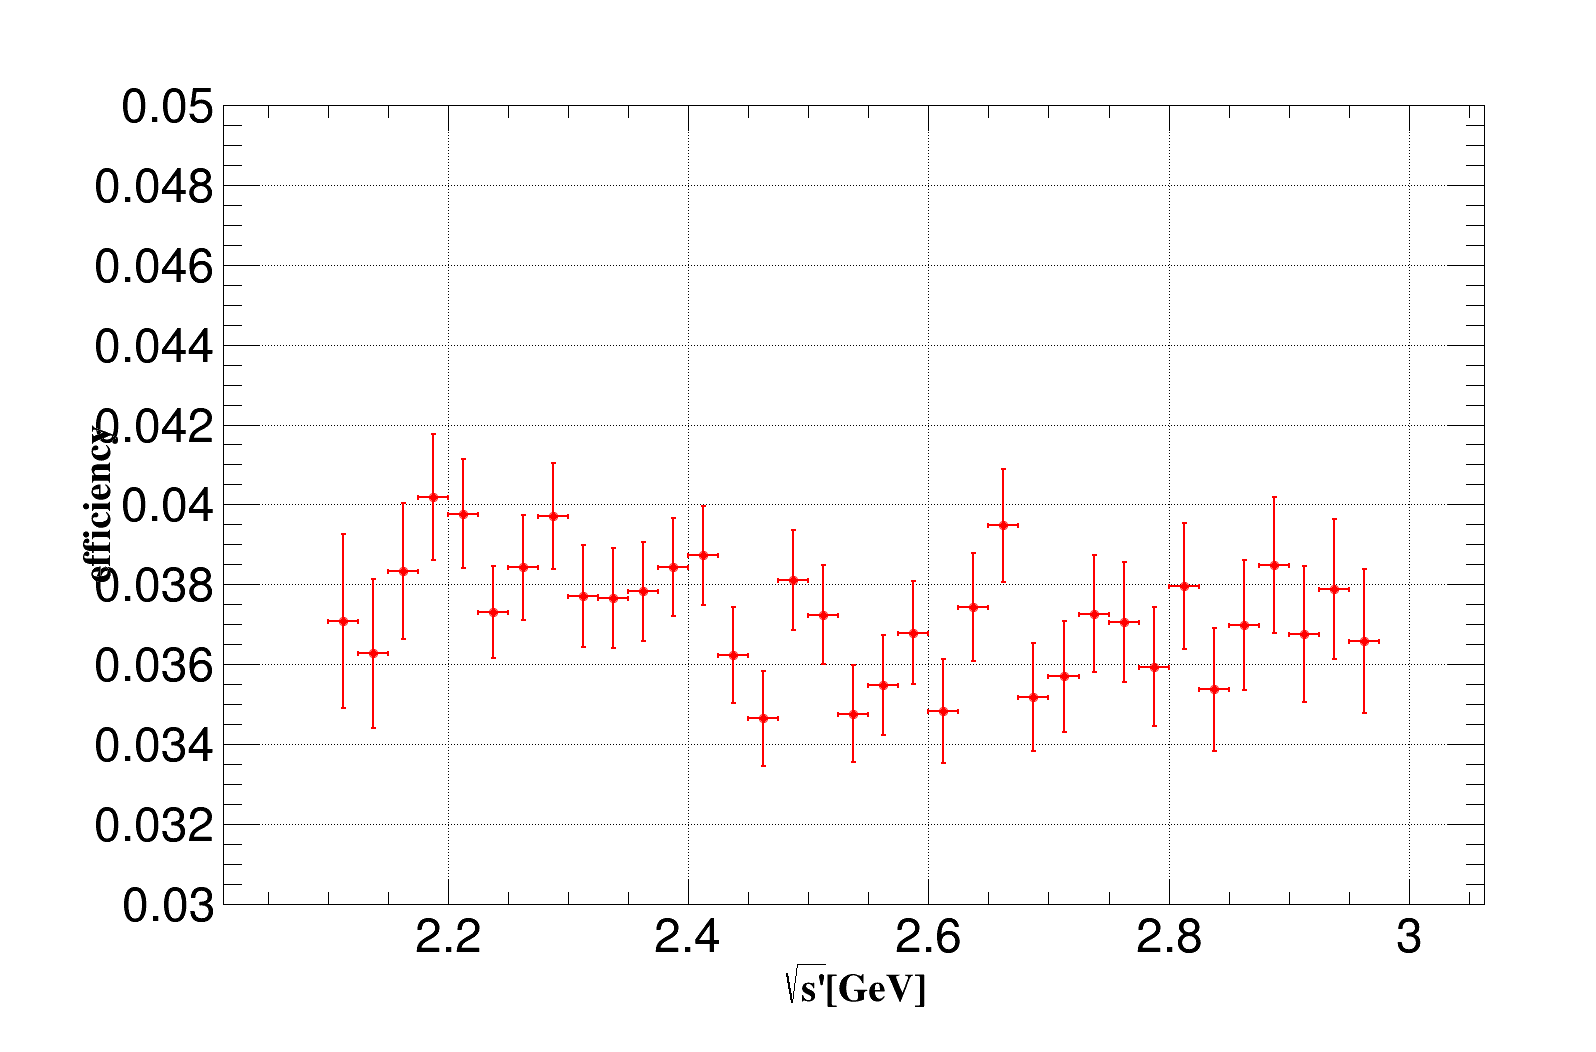
\includegraphics[width=\textwidth]{figures/1b36c40nphi_efficiency.png}
  \end{column}
 \end{columns} 
\end{frame}


\begin{frame}
  \frametitle{Simulation vs Data}
  \begin{columns}
    \begin{column}{0.5\textwidth}
      \centering
      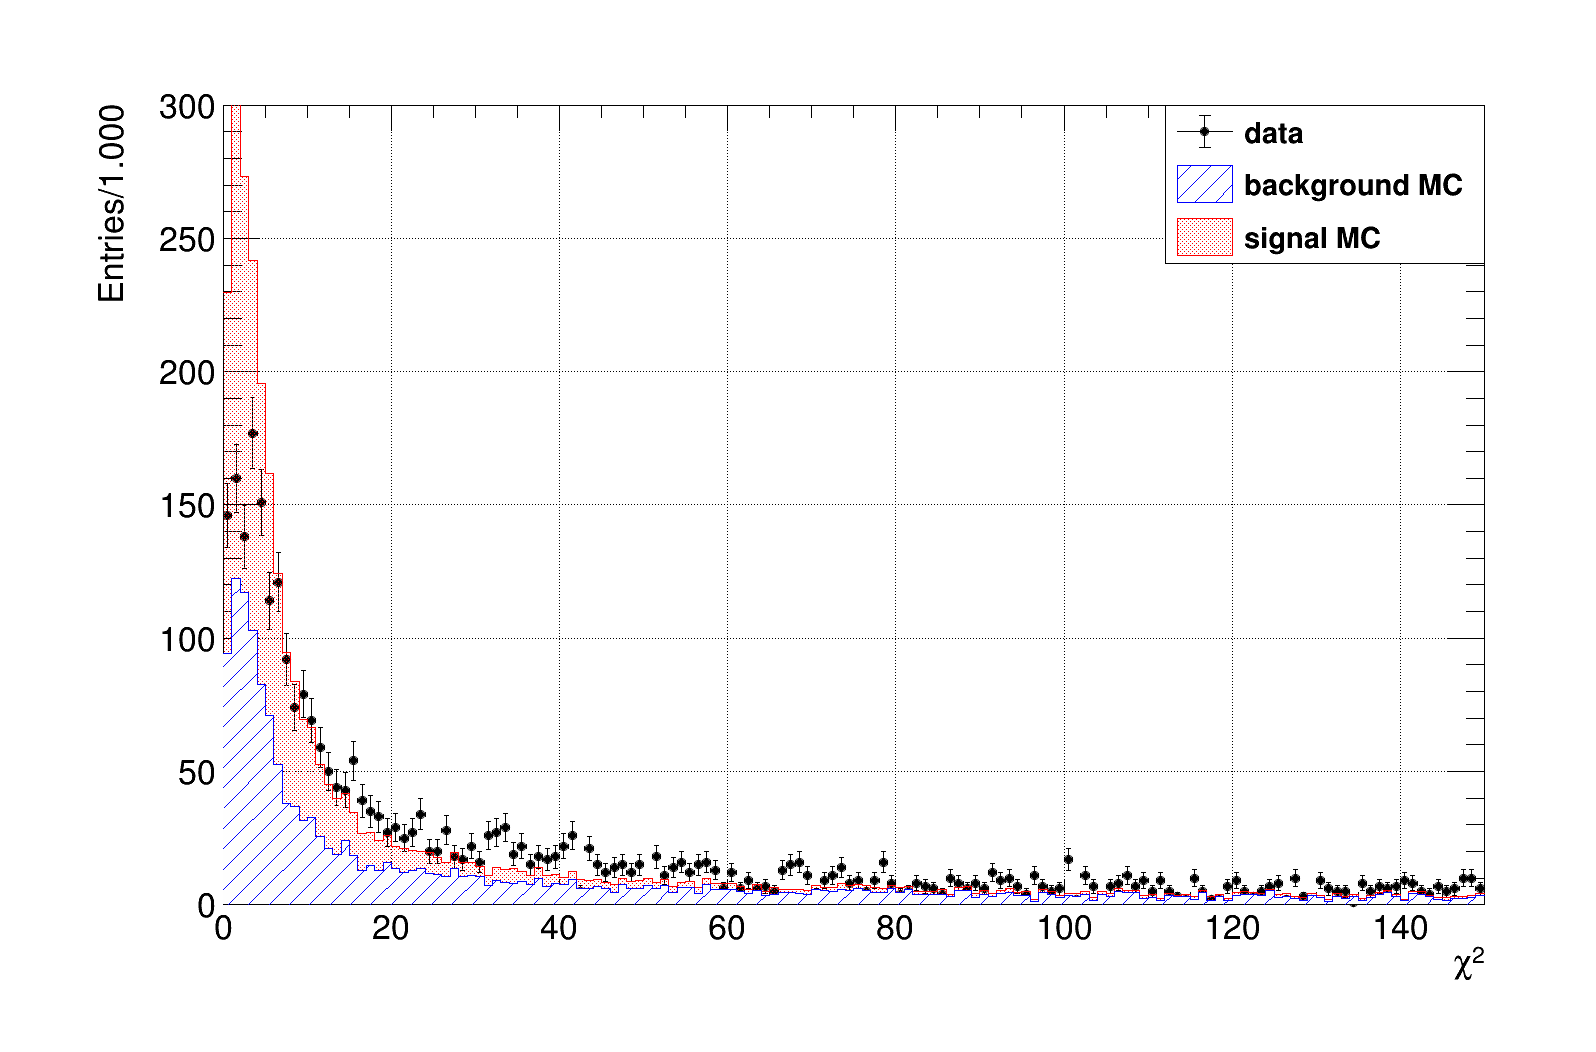
\includegraphics[width=\textwidth]{figures/data_vs_mc_chisq.png}
    \end{column}

    \begin{column}{0.5\textwidth}
      \centering
      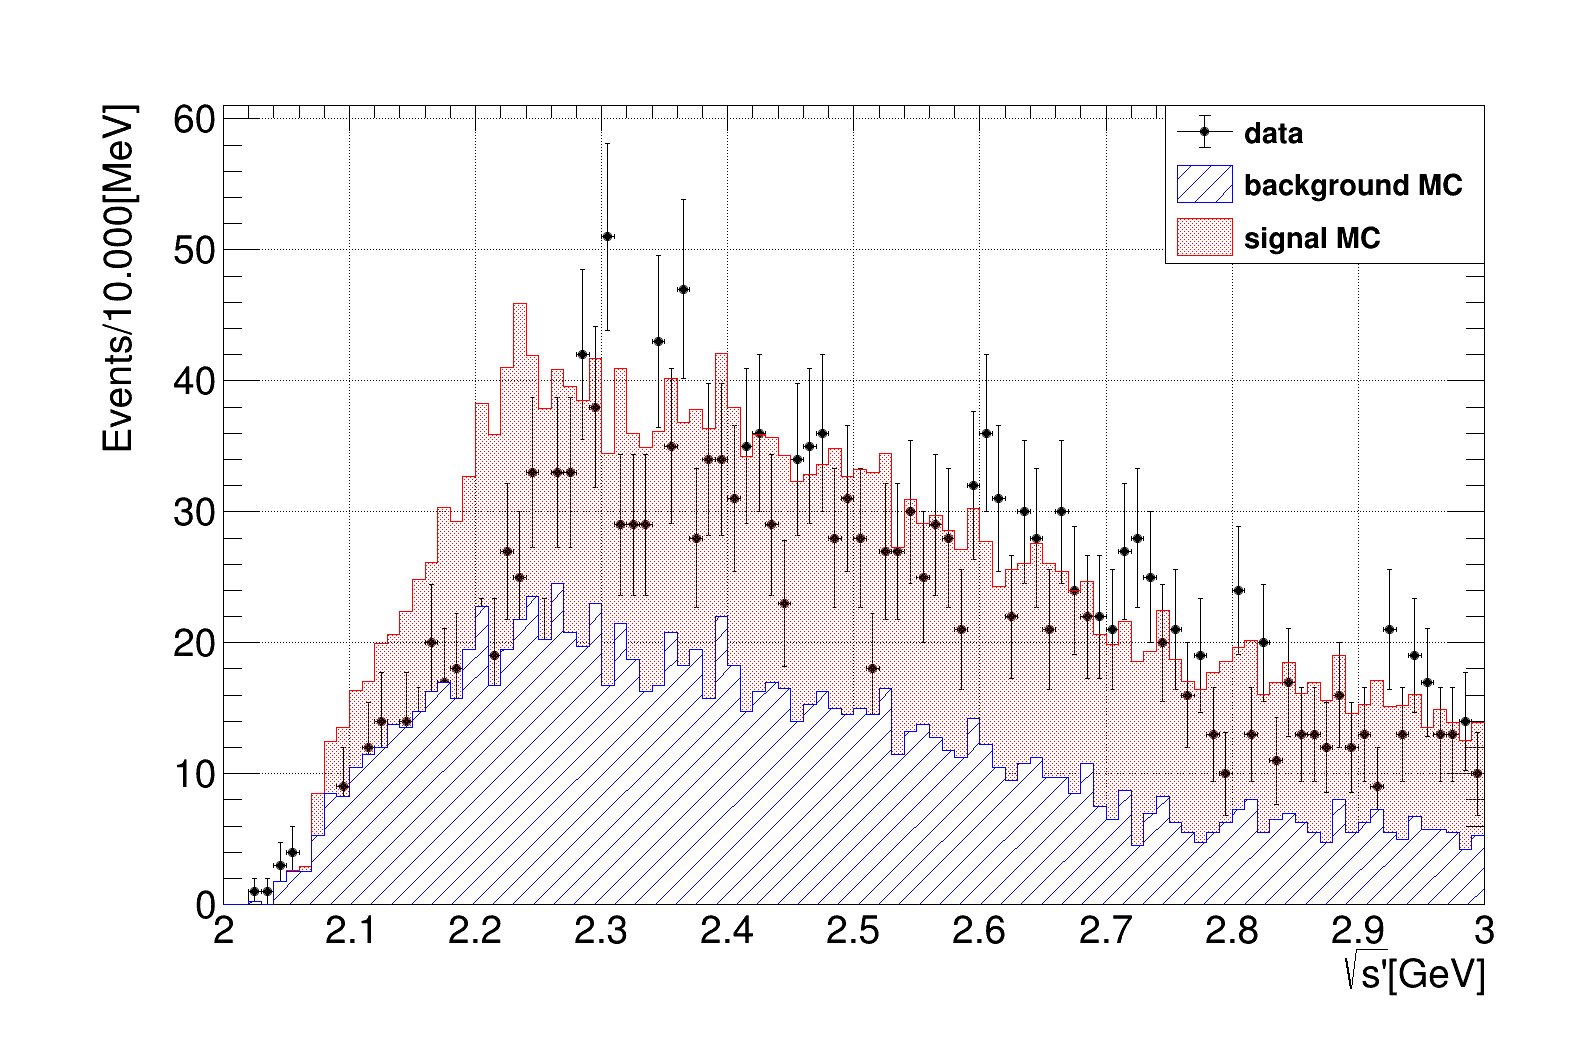
\includegraphics[width=\textwidth]{figures/data_vs_mc_vpho.png}
    \end{column}
  \end{columns}
\end{frame}

\section{Branch Fraction of $J/\psi\to K^+ K^-$}


\section{Summary}


\section*{Back up}

\begin{frame}
  \begin{itemize}
    \item[$\star$] 暂时存在的一些问题:
    \begin{itemize}
    \item Data-Driving 去除本底的方式只适用于Born过程,在这里出现的主要峰状本底是$e^+e^-\to \phi \phi \gamma^I$,此方式并不合适
    \item 关于PID的优化在与又文讨论后在细节上还存有一点问题,需进一步讨论
    \end{itemize}

    \item[$\star$] to do list:
    \begin{itemize}
      \item 产生run-dependent 的signalMC ?
      \item 搞清$J/\phi$ 分支比验证的流程
      \item 其他能区的分析
    \end{itemize}


    
  \end{itemize}
\end{frame}

\end{document}
